%!TEX root = ./Thesis.tex

\chapter{Experimental engineering of qudit states}
\label{chapter:experimental_engineering_qudits}

\tmpHeading{Summary of the work} In this section we present an experimental implementation of the state engineering scheme discussed in~\cref{chapter:quantum_walks}, which, leveraging the \emph{coin space} of a \ac{QW} as an auxiliary degree of freedom, allows to engineer target qudits over a fixed number dimensions.
More specifically, we use an experimental apparatus implementing time-dependent \acp{QW} in the polarisation and \ac{OAM} degrees of freedom~\cite{zhang2010implementation,goyal2013implementing,cardano2015quantum}, exploiting the so-called \acp{QP}~\cite{marrucci2006optical}, to couple the OAM and polarisation degrees of freedom of light.
The work described in this chapter can be found in~\cite{giordani2019experimental}.

\tmpHeading{Why \ac{OAM}?} \acf{OAM} offers the possibility to encode high-dimensional quantum states in spatially localised photons. Moreover, \acp{QP} intertwine the polarisation and \ac{OAM} degrees of freedom of light, thus allowing more complex dynamics exploiting both types of degrees of freedom.
With this apparatus, $n$ \ac{QW} steps require $\mathcal O(n)$ optical components -- one \ac{QP} and a few waveplates for each step -- thus making the scheme efficient. Moreover, by having access to fast-enough optical switches and fastly tunable \acp{QP} and waveplates, it is in principle possible to use a single \ac{QP} and waveplate for arbitrary many steps, by having the light pass through the same optical elements multiple times \highlight{(mmmh)}.
% in \emph{light} of the favourable scaling of the number of optical elements with the size of the walk~\cite{reck1994experimental,clements2016optimal}. Moreover, the scheme allows for the full control of the coin operation that is key to the walk implementation of the walk.


\tmpHeading{What will we conclude from the chapter?}
The quality of the generated states and the feasibility of the experimental protocol that we have put in place, demonstrate the effectiveness of a hybrid platform for quantum state engineering. Such platform holds together a programmable quantum system, the photonic \ac{QW} in the angular momentum, and classical optimization algorithms to effectively generate a given target \highlight{???}.

\tmpHeading{Outline of chapter}
In~\cref{sec:expQWs:OAMintro} we give a brief overview of orbital angular momentum states of light and vector vortex beams.
In~\cref{sec:expQWs:engineeringQWs} we review the results obtained in~\cref{chapter:quantum_walks} that are relevant to the present chapter, and provide more background for the type of states generated \highlight{(unless I change my mind about the latter)}. The experimental details are then reported in~\cref{sec:expQWs:experimental_apparatus}. \highlight{(To finish upon chapter completion)}


\section{Orbital angular momentum of light}
\label{sec:expQWs:OAMintro}

\tmpHeading{Orbital angular momentum of light}
Electromagnetic fields carry angular momentum~\cite{jackson1999classical}.
Classically, the angular momentum density of an electromagnetic field is given, up to constants, by
$\bs M =\bs r\times(\bs E\times \bs B)$. This can be decomposed in an \emph{intrinsic} component, the so-called \emph{spin angular momentum}, and an \emph{extrinsic} one, its \acp{OAM}: $\bs M=\bs S+\bs L$, albeit this distinction turns out to not be gauge invariant, and thus comes with its own problems~\cite{ohanian1986what,cameron2015azimuthal}.
The spin angular momentum is often understood to be due to an internal degree of freedom of the fields, while the OAM is due to its spatial profile structure.
A first experimental demonstration of transfer of \emph{spin} angular momentum of light to matter was given in~\cite{beth1936mechanical}. A few decades later, Allen and collaborators showed that that specific types of laser modes also carry an amount of \emph{orbital} angular momentum, due to nontrivial phase structures of their transverse beam profile~\cite{allen1992orbital}.
Despite the Poynting vector $\bs E\times \bs B$ always pointing in the propagation direction for transverse beams, and thus $\bs r\times(\bs E\times\bs B)$ being vanishing in such direction, Allen et al. realised that the TEM$_{p\ell q}$ laser modes are in general \emph{not} transverse, but rather have a component in the propagation direction. Because of this, they could show that, for this fields, $\bs M$ has a component in the propagation direction that is proportional to $\ell$, which is the quantum number that determines the azimuthal phase profile of the field.
Since Allen's ground breaking paper, the OAM degree of freedom of light has been showed to be useful for a variety of applications in quantum information theory~\cite{allen1999orbital,padgett2004lights,barnett2007orbital,franke-arnold2008advances,yao2011orbital,padgett2017orbital,erhard2017twisted}, as a notable example, entanglement in the OAM degree of freedom of photons was first demonstrated in~\cite{mair2001entanglement}.

\tmpHeading{Laguerre-Gauss beams}
The most common type of helical laser beams carrying OAM are \ac{LG} modes $LG_p^\ell$. These modes arise from solving the Helmholtz equation in cylindrical coordinates in the paraxial approximation. The main feature of these beams that will be used in the context of our work is their azimuthal phase dependence: $LG_p^\ell\sim e^{i\ell\phi}$ with $\phi$ the azimuthal coordinate in the plane transverse to the propagation direction.
\highlight{(should I show more explicitly how LG modes come from the equations?)}

\tmpHeading{Coupling OAM with polarisation}
Whereas in the vacuum the spin and orbital components of the angular momentum are conserved, this ceases to be the case in inhomogeneous, anisotropic media. This makes it possible to devise devices which couple spin and orbital angular momenta of an incoming state. One such device is the so-called \ac{QP}~\cite{marrucci2006optical}.
When a nontrivial phase dependence is coupled with a helicoidal transverse polarisation pattern, one talks of a \ac{VVB}~\cite{cardano2012polarization}. These can be generally described as states in which different polarisation states of light are coupled with different OAM states.
The interest in such states is motivated by the applications in multiple fields of classical and quantum optics~\cite{marrucci2011spintoorbital,cozzolino2019highdimensional}: from particle trapping to metrological applications in microscopy~\cite{cardano2015spin–orbit,rubinsztein-dunlop2016roadmap}, and for \ac{OAM}-based communications schemes in free-space and in-fibre~\cite{willner2015optical,cozzolino2019aircore}.
\acp{VVB} are also often employed in quantum information protocols due to the hyperentanglement between their polarisation and spatial degrees of freedom. Photonic platforms for quantum sensing and metrology leveraging such encoding have also been reported~\cite{fickler2012quantum,dambrosio2013photonic}. VVB-based schemes for investigating quantum causal structures~\cite{goswami2018indefinite}, quantum communication and cryptography~\cite{vallone2014freespace,wang2015quantum,mirhosseini2015highdimensional,malik2016multiphoton,sit2017highdimensional,cozzolino2019orbital}, quantum walks~\cite{zhang2010implementation,goyal2013implementing,cardano2015quantum}, quantum simulation~\cite{cardano2016statistical,cardano2017detection}, quantum memories~\cite{parigi2015storage}, and quantum state engineering~\cite{innocenti2017quantum,giordani2019experimental}, have all been previously demonstrated. 

\tmpHeading{Open questions with VVBs}
Despite the potential of \acp{VVB}, many questions regarding the decoding of information stored in \ac{OAM} and polarisation remain unanswered. Various techniques of \ac{OAM}-demultiplexing envisage the need of additional instruments -- such as interferometry~\cite{leach2002measuring,slussarenko2010polarizing,bauer2013nanointerferometric} or spatial filtering~\cite{berkhout2010efficient,bolduc2013exact,malik2014direct} -- to be efficiently implemented.
These introduce detrimental effects of loss and noise~\cite{qassim2014limitations}. Moreover, the challenge of performing state tomography in such a high-dimensional framework, a fundamental task in quantum information processing~\cite{paris2004quantum,banaszek2013focus}, can hardly be overestimated. The design and demonstration of reliable techniques for the generation and classification of~\acp{VVB} is thus highly desirable. Indeed, substantive efforts on finding novel platforms are subject of intense research activities~\cite{liu2016generation,ndagano2017creation,cardano2015spin–orbit,rubinsztein-dunlop2016roadmap},
including in integrated photonics~\cite{chen2018mapping,cai2012integrated,liu2017direct} and generation by plasmonic metasurfaces~\cite{karimi2014generating,yue2016vector}.


\begin{figure}[tb]
	\centering
	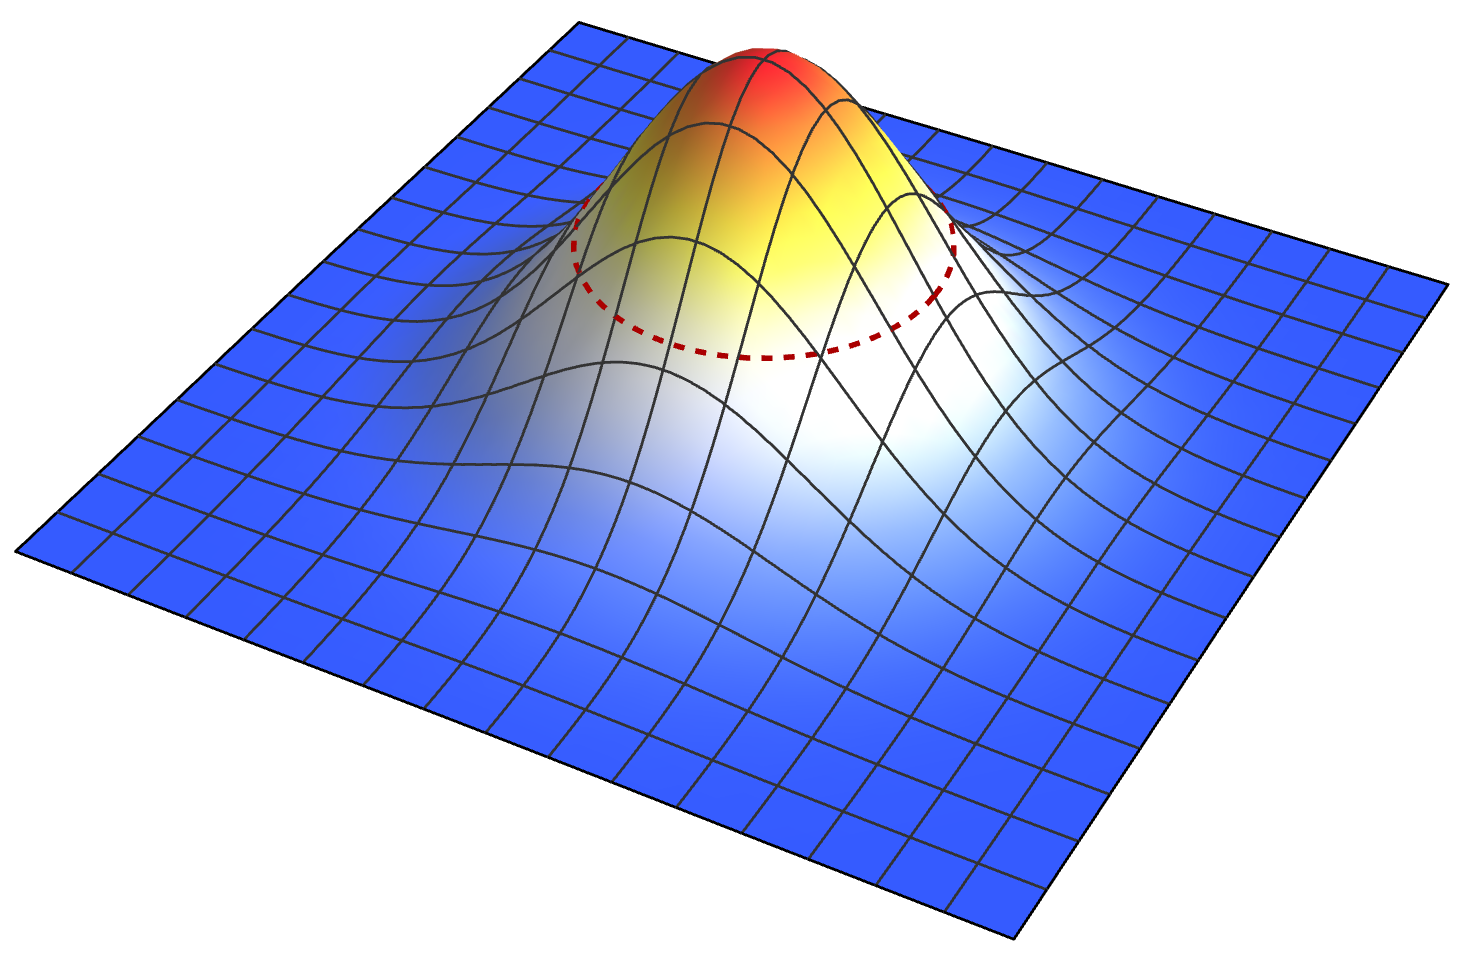
\includegraphics[width=.7\linewidth]{Figures/OAM/GaussianBeam2.png}
	\caption{%
		Gaussian beam
	}
	\label{fig:expQWs:gaussian_beam}
\end{figure}

\begin{figure}[tb]
	\centering
	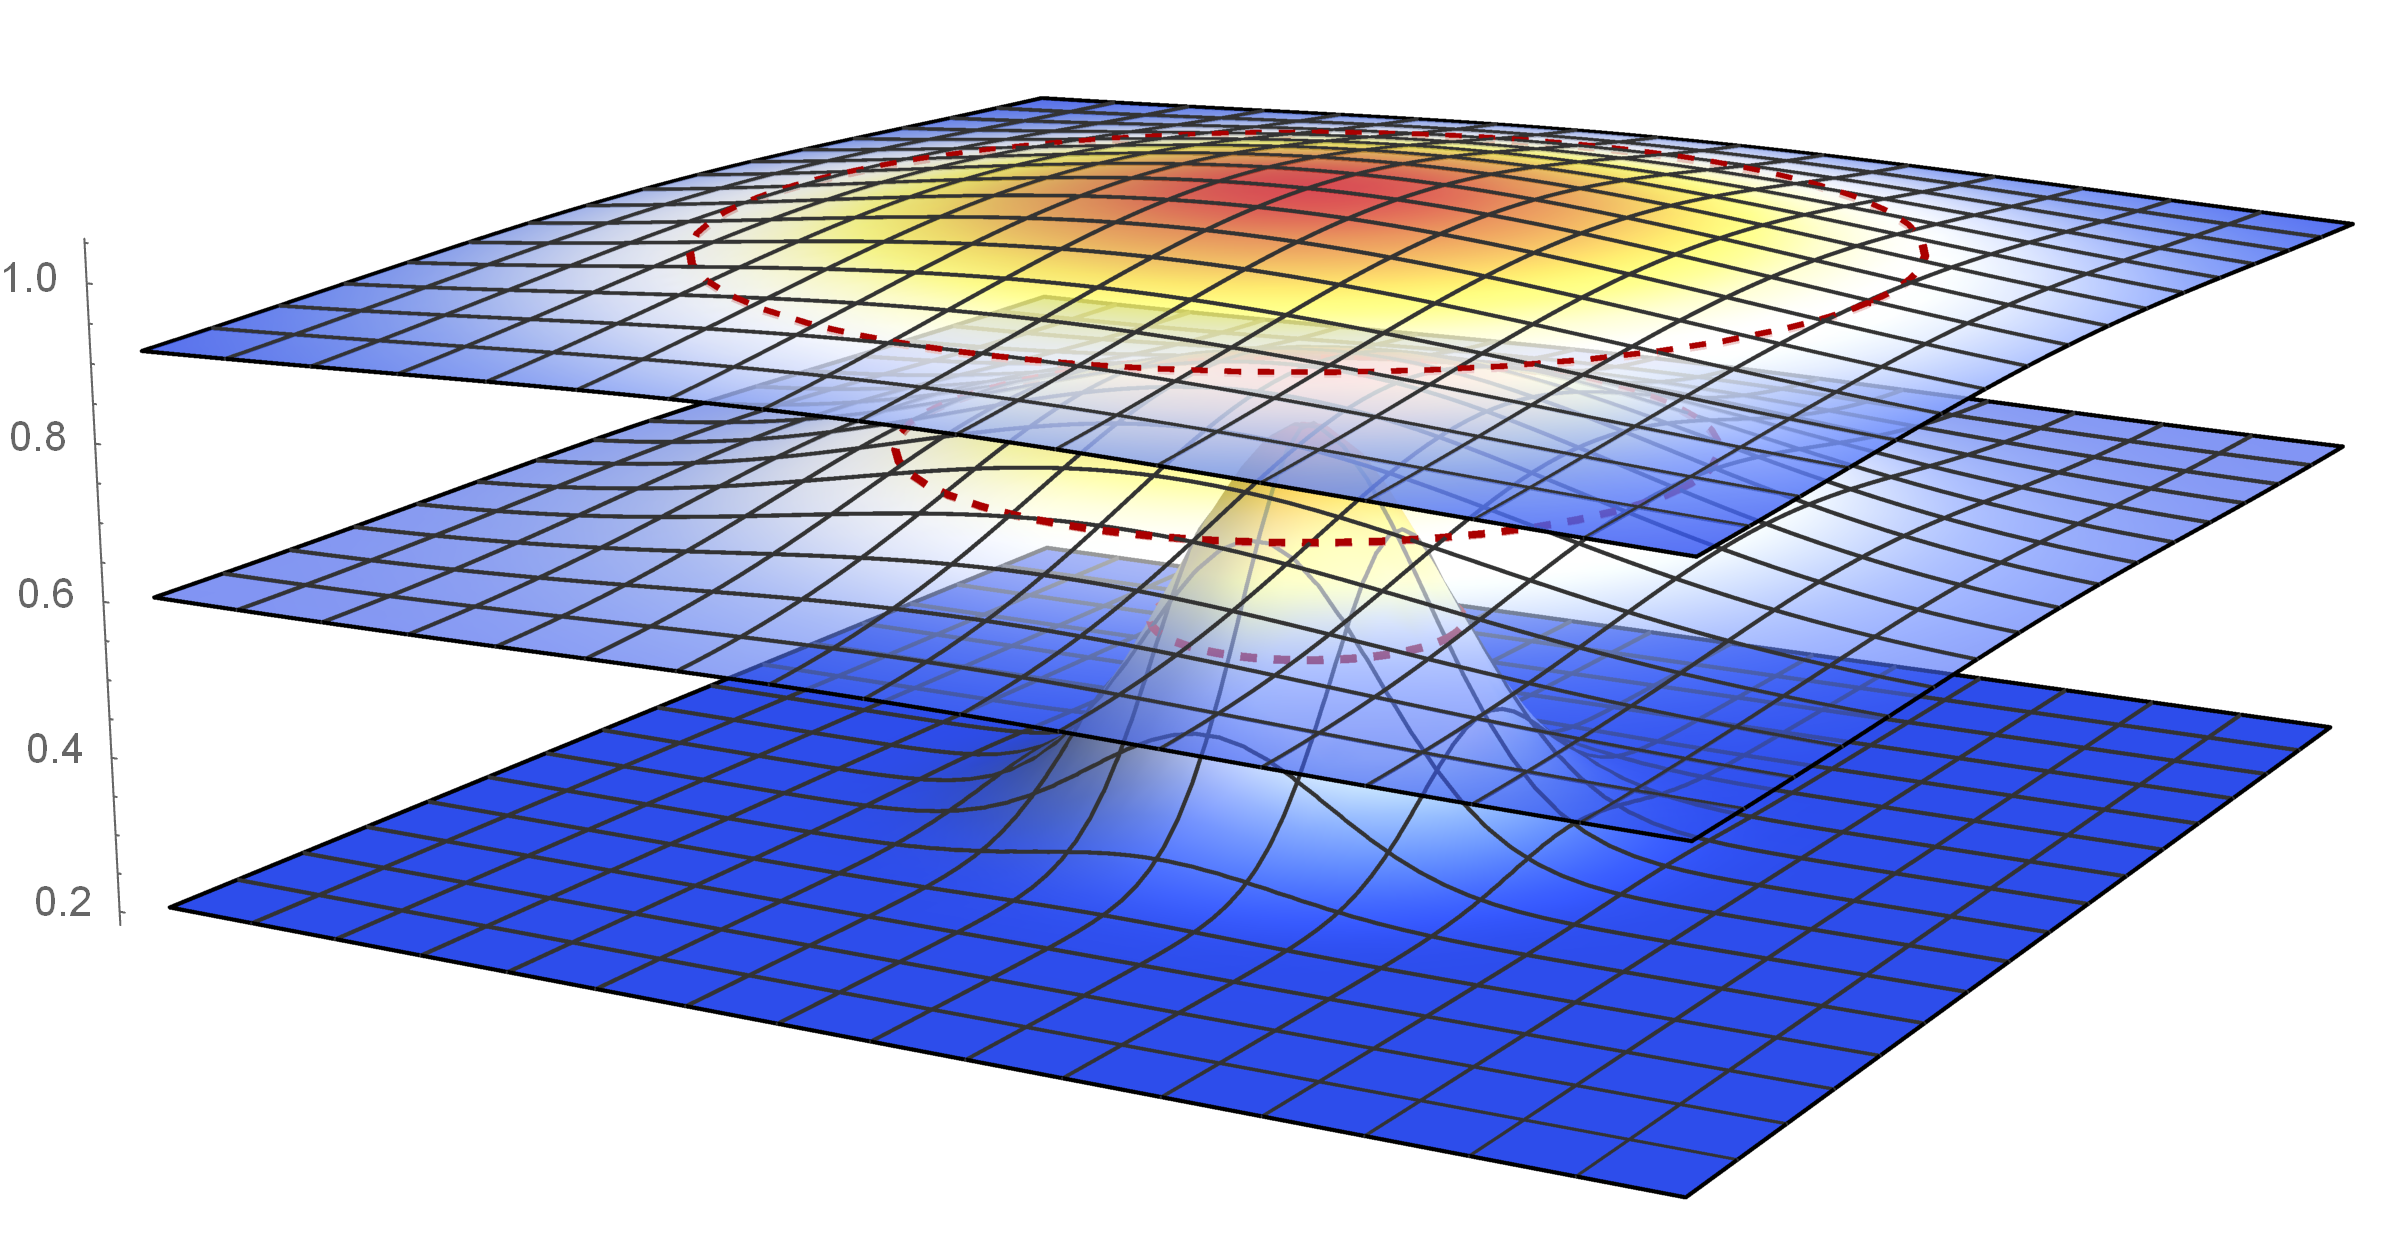
\includegraphics[width=.7\linewidth]{Figures/OAM/GaussianBeamDispersion.png}
	\caption{%
		Gaussian beam
	}
	\label{fig:expQWs:gaussian_beam}
\end{figure}

\begin{figure}
    \centering
    \begin{minipage}{0.45\textwidth}
        \centering
        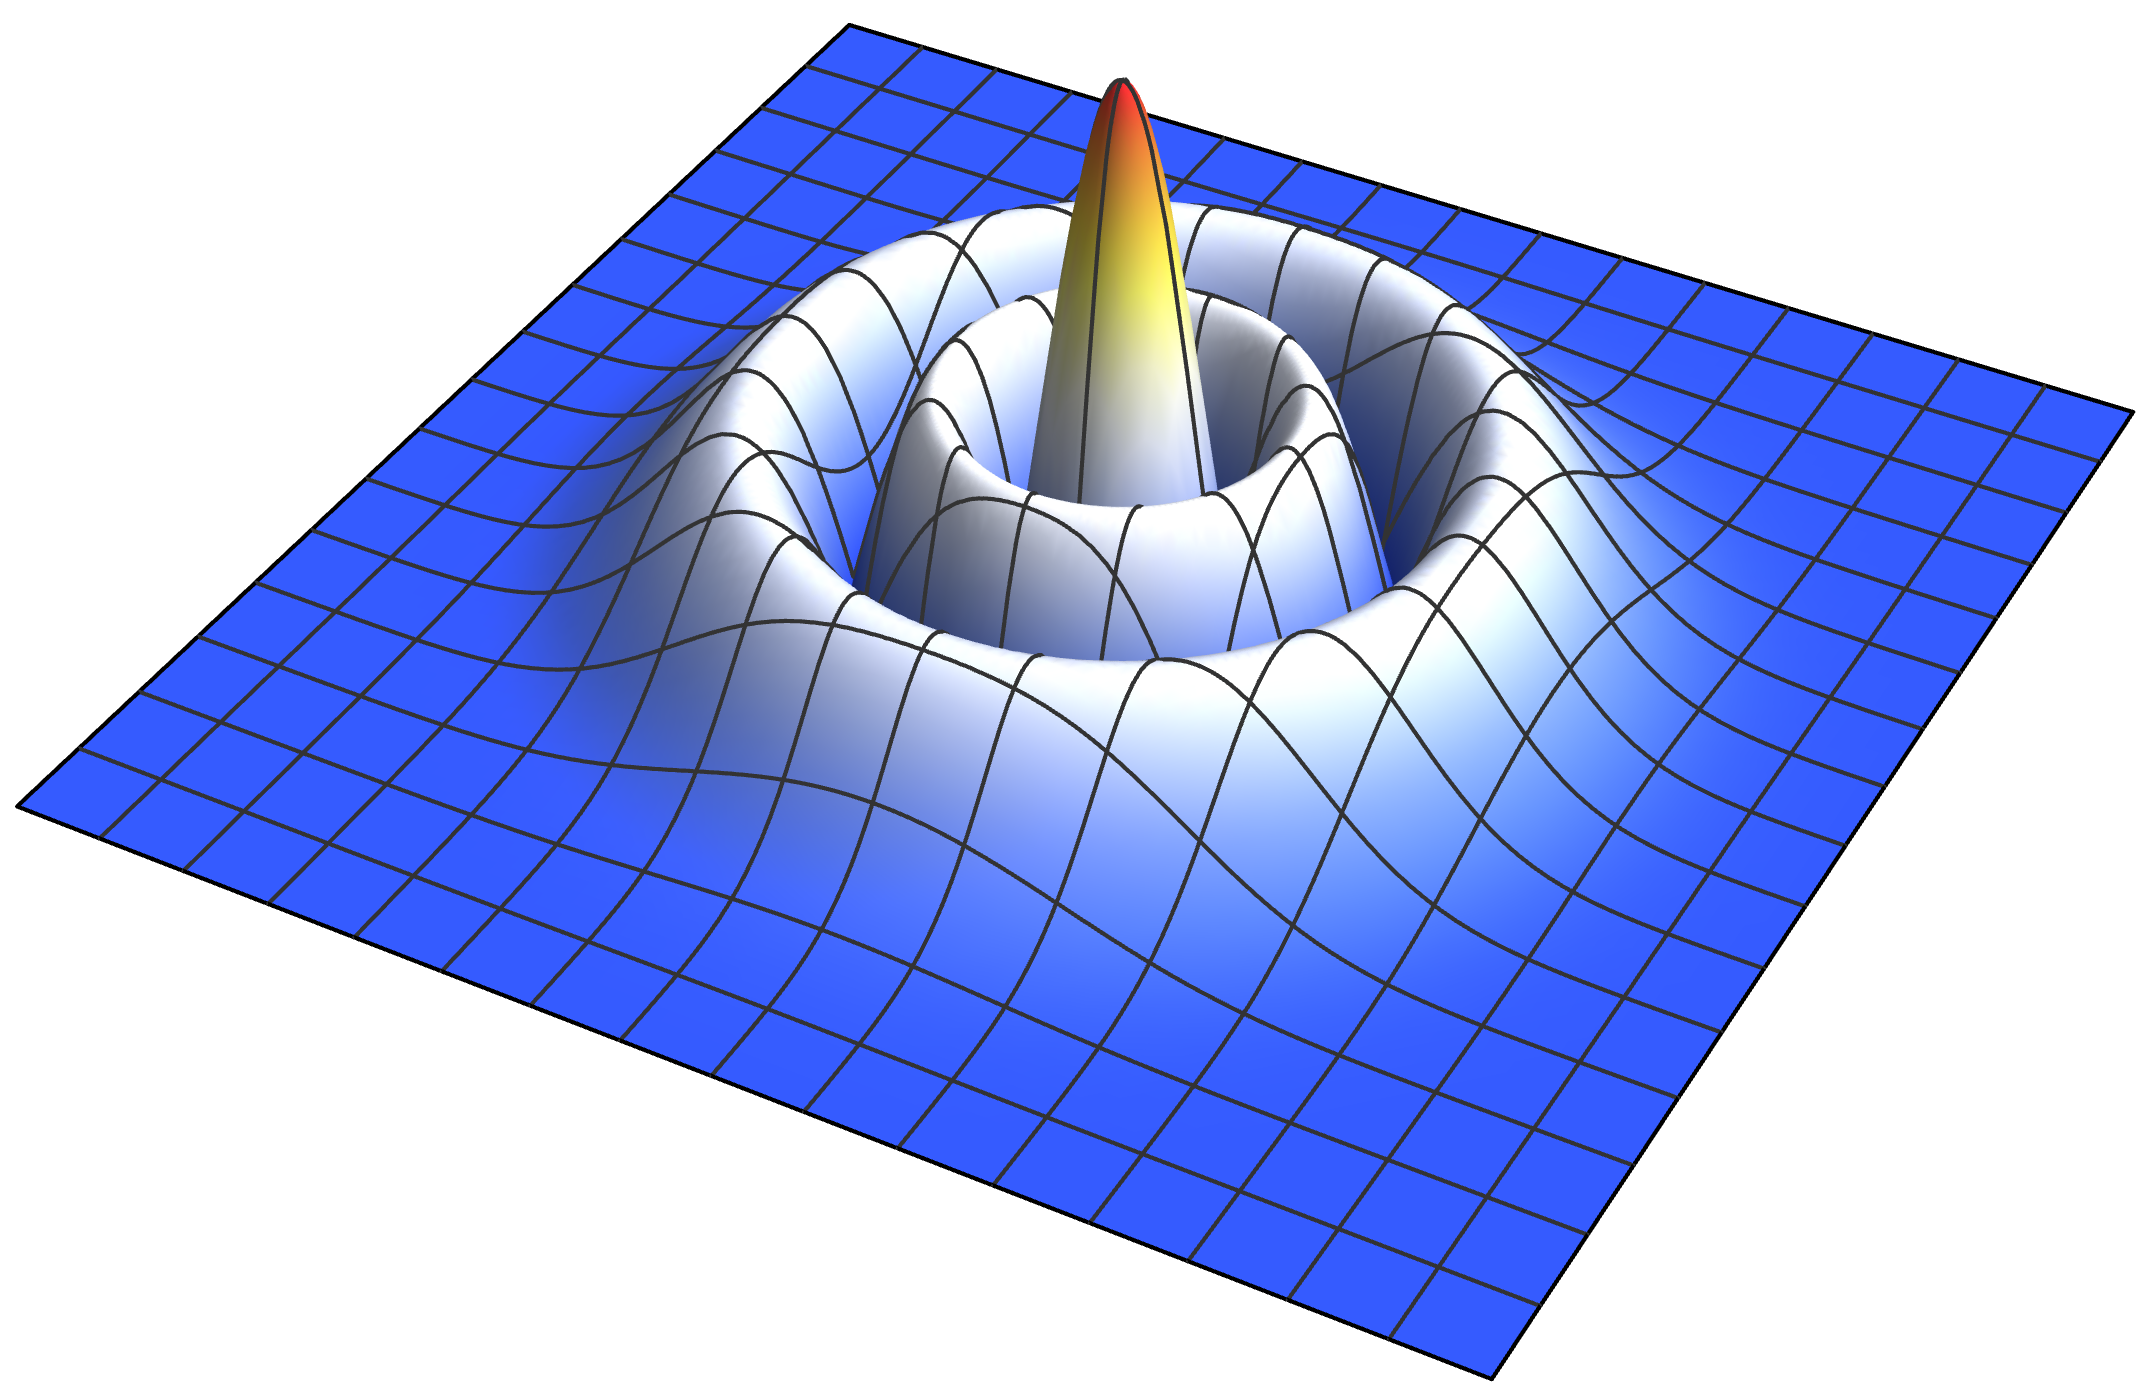
\includegraphics[width=1\textwidth]{Figures/OAM/LGBeamProfile_L0P2Z03.png} % first figure itself
        \caption{first figure}
        \label{fig:expQWs:gaussian_profile_L0P2Z03}
    \end{minipage}\hfill
    \begin{minipage}{0.45\textwidth}
        \centering
        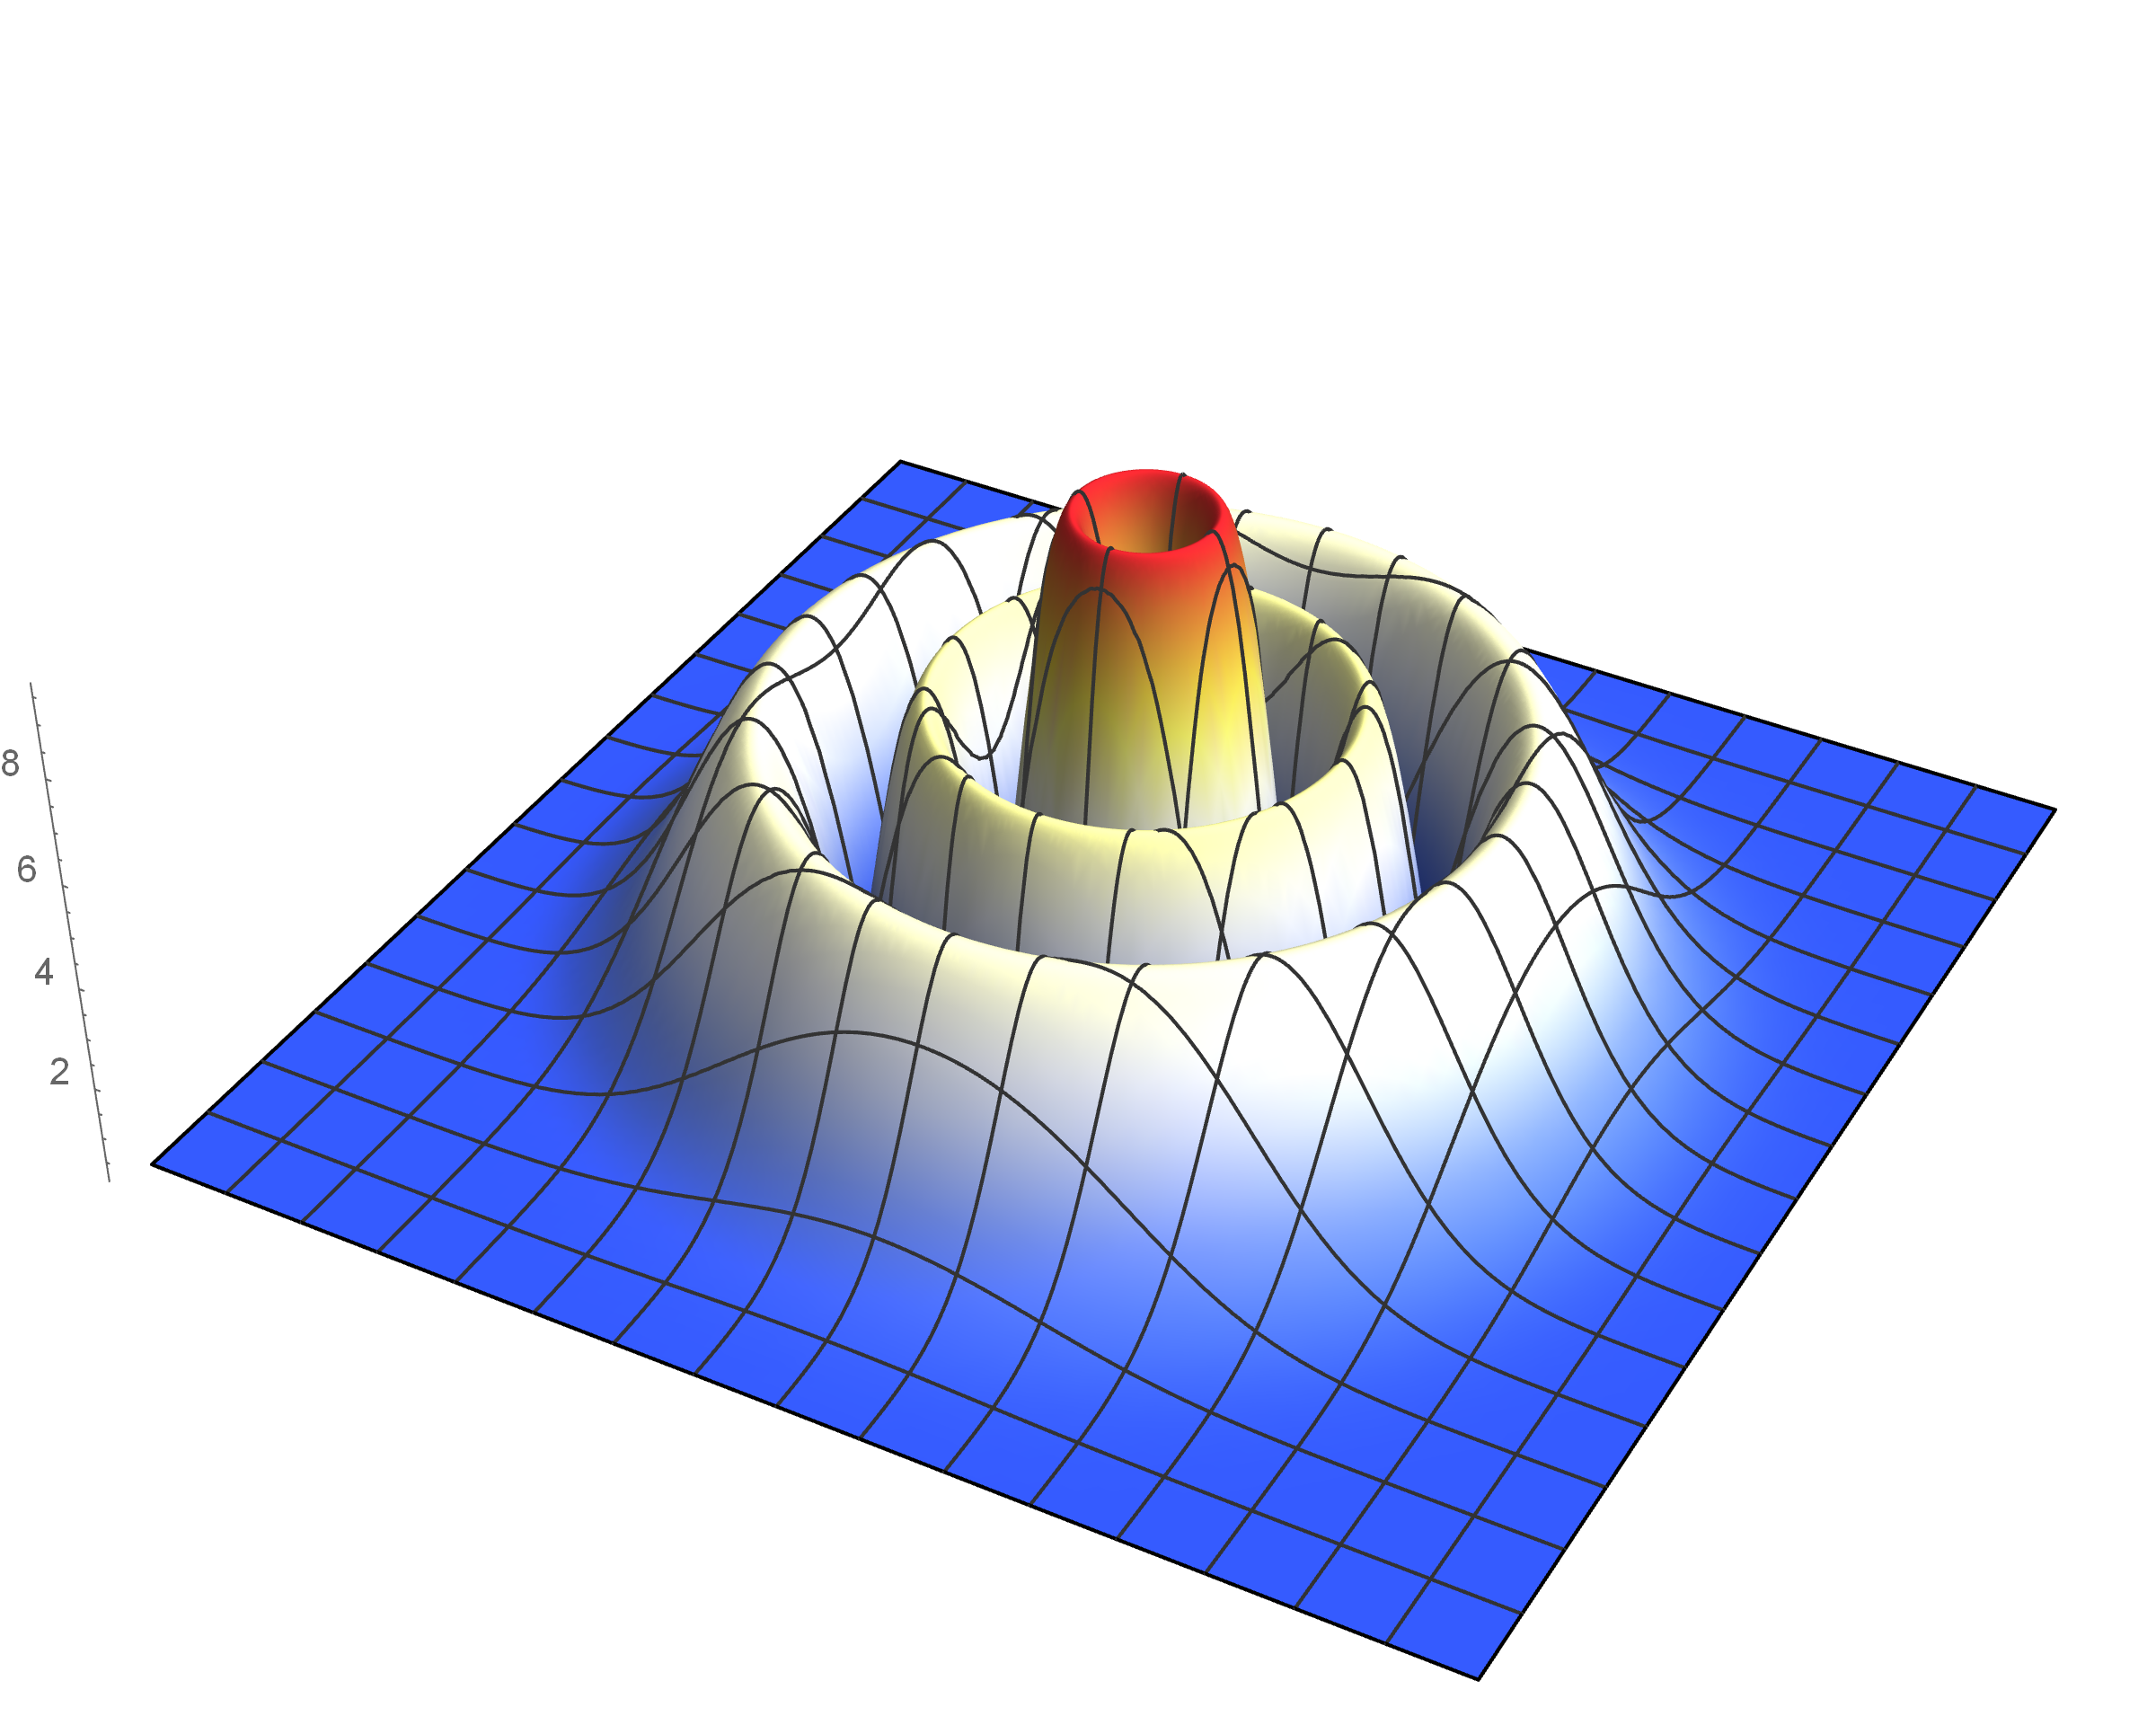
\includegraphics[width=1\textwidth]{Figures/OAM/LGBeamProfile_L1P2Z03.png} % second figure itself
        \caption{second figure}
        \label{fig:expQWs:gaussian_profile_L1P2Z03}
    \end{minipage}
\end{figure}

\FloatBarrier
\section{State engineering protocol}
\label{sec:expQWs:engineeringQWs}

\tmpHeading{How do we generate qudits via QWs?}
In~\cref{chapter:quantum_walks}, and more specifically in~\cref{sec:QWs:reachability_conditions,sec:QWs:focusing_walker_states}, we showed that arbitrary qudits of dimension $N+1$ can be generated via a \ac{DTQW} dynamics with suitably chosen coin operations and coin projection at the end of the walk. Here, we present an experimental implementation of this protocol, showcasing in a few relevant scenarios that computing and implementing the necessary coin operations and projection is in fact practical in an experimental photonic context.

% We consider a discrete-time \ac{QW} with a two-dimensional coin with logical states labelled as $\{\ket{\downarrow}_c, \ket{{\uparrow}}_c\}$. The dynamics are made up of consecutive unitary steps. At step $t$, a \emph{coin operator} $\hat{\mathcal{C}_{t}}$ changes the coin state and is then followed by a \emph{shift operator} $\calS$, which moves the walker conditionally to the coin state. Such transformations are described by the operators
% \begin{equation}
% 	\hat{\mathcal{C}_t}=
% 	\left(
% 	\begin{array}{ll}
% 	e^{i \xi_t} \cos{\theta_t} &  e^{i \zeta_t} \sin{\theta_t} \\
% 	-e^{-i \zeta_t} \sin{\theta_t} & e^{-i \xi_t} \cos{\theta_t}
% 	\end{array}
% 	\right),
% \end{equation}
% which accounts for the coin tossing, and
% $\calS=\sum_k |k-1\rangle \langle k|_w\otimes |{\downarrow}\rangle \langle {\downarrow}|_c+ |k+1\rangle \langle k|_w\otimes |{\uparrow}\rangle \langle{\uparrow}|_c$,
% which realizes the conditional motion of the walker. Here $k$ is the lattice-site occupied by the walker and $\{\theta_t,\xi_t,\zeta_t \}$ are parameters identifying a unitary transformation in two dimensions. The evolution through $n$ steps of the {QW} is given by $\hat{U}=\prod_{t=1}^n \calS\hat{\calC_t}$.

% In~\cite{innocenti2017quantum} it was shown that it is always possible to find a set of coin operators $\{\hat{\mathcal{C}_t}\}_{t=1}^{n}$ that produce an arbitrary target state in the full coin-walker space. In addition, via suitable projection in the coin space, arbitrary walker states can also be obtained. The identification of the correct set of coin operators is enabled by a classical algorithm to maximize the fidelity between the final state of the walker, after projection of the coin, and the target $(n+1)$-dimensional state. It is worth noting that all states can be reachable with unit fidelities (albeit probabilistically) and high probabilities, regardless of the number of steps $n$ (see Ref.~\cite{SI}).


\tmpHeading{What states do we generate?}
We demonstrate the experimental engineering of arbitrary six-dimensional qudits using a five-step \ac{DTQW}. We focus on a few physically relevant classes of states: \emph{angular-momentum Schrödinger cat states}, \emph{spin-coherent states}, as well as completely balanced and randomly sampled states.

\emph{Angular-momentum Schrödinger cat states}~\cite{militello2006distilling} are here understood as superpositions of extremal walker positions. The correspondence between the position space of the walker and an angular momentum of quantum number $n/2$, which will be explained later in this section, makes the \ac{QW} perfectly suited to synthesise this class of states. Schrödinger cat states play a crucial role in the investigations on foundations of quantum mechanics~\cite{schrodinger1935gegenwartige}\highlight{sbadabem} and their generation is at the core of various quantum engineering protocols~\cite{brune1992manipulation, monroe1996schrodinger,agarwal1997atomic, zhang2016creating}. The second class of states that we consider are \emph{spin-coherent states}~\cite{ulyanov1999spin}, which are the spin-like counterpart of \emph{coherent states} of a quantum harmonic oscillator. Finally, in order to validate the flexibility of our approach, we demonstrate high-quality engineering of both balanced, and randomly sampled states \highlight{(These details might be better suited on their own sections)}.

\section{Experimental apparatus}
\label{sec:expQWs:experimental_apparatus}

\tmpHeading{Experimental implementation of QW}
We implement a \ac{DTQW} with $n=5$ steps, using \ac{OAM} as the physical embodiment of the \emph{walker} degree of freedom, and the polarisation as the \emph{coin}.
% are encoded in circular-polarisation states $\{|R\rangle, |L\rangle\}$. We dub such degree of freedom as \ac{SAM} to mark the difference with \ac{OAM}.
Our experimental setup, which is shown schematically in Fig.~\ref{fig:expQWs:schematics} and follows Refs.~\cite{cardano2015quantum,cardano2016statistical}, allows for the full coin-walk evolution to take place in a single light beam, thus avoiding a nonlinear growth of optical paths as in previous interferometric implementations~\cite{zhang2010implementation,goyal2013implementing,cardano2015quantum}. Such scheme guarantees a linear scaling of the number of optical elements needed to implement a $n$-step \ac{QW} (see Ref.~\cite{SI}). Arbitrary coin operators are achieved through a sequence of suitably arranged \ac{QWP} and \ac{HWP}~\cite{simon1990minimal}. The shift operator $\calS$ is implemented using a \ac{QP}~\cite{marrucci2006optical}, a birefringent liquid-crystal medium that rises and lowers the value of the \ac{OAM} conditionally to the polarisation~\cite{marrucci2006optical}. More specifically, \acp{QP} act on \ac{OAM} states with azimuthal quantum number $m$ and polarisation $\ket L$ or $\ket R$ as follows:
\begin{equation}
\begin{aligned}
	\ket{L,m} & \xrightarrow{\text{QP}} \cos(\delta/2) \ket{L,m}
									&+& i e^{2 i \alpha_0} \sin(\delta/2) \ket{R,m+2q}, \\
	\ket{R,m} & \stackrel{\text{QP}}{\longrightarrow} \cos(\delta/2) \ket{R,m}
									&+& i e^{-2 i \alpha_0} \sin(\delta/2) \ket{L,m-2q},
\end{aligned}
\end{equation}
where $q$ is the so-called \emph{topological charge} of the device.
The additional phase $\alpha_0$ between the two polarisations is compensated by changing the orientations of the waveplates which implement the coin operator of the subsequent step.
By suitable choice of $\delta,\alpha_0$, the QP can therefore be made to act as
$\ket{R,m}\xrightarrow{\text{QP}} \ket{L,m-2q}$ and $\ket{L,m}\xrightarrow{\text{QP}}\ket{R,m+2q}$, where $q$ is the topological charge of the \ac{QP}.

Measurement of the coin in the $\ket+$ state is performed with a \ac{HWP} and a \ac{PBS}, while the \ac{OAM} state can be analysed with a \ac{SLM}~\cite{cardano2015quantum}.
Therefore, the \ac{DTQW} is made up of consecutive optical units composed of wave plates (coin operators) and a QP (shift operators).
The number of optical elements scales polynomially with the number of steps, making this scheme scalable.
Finally, a \ac{SLM} can be also employed before the \ac{QW} architecture to prepare the initial walker state spanning $n$ sites.


\begin{figure}[tb]
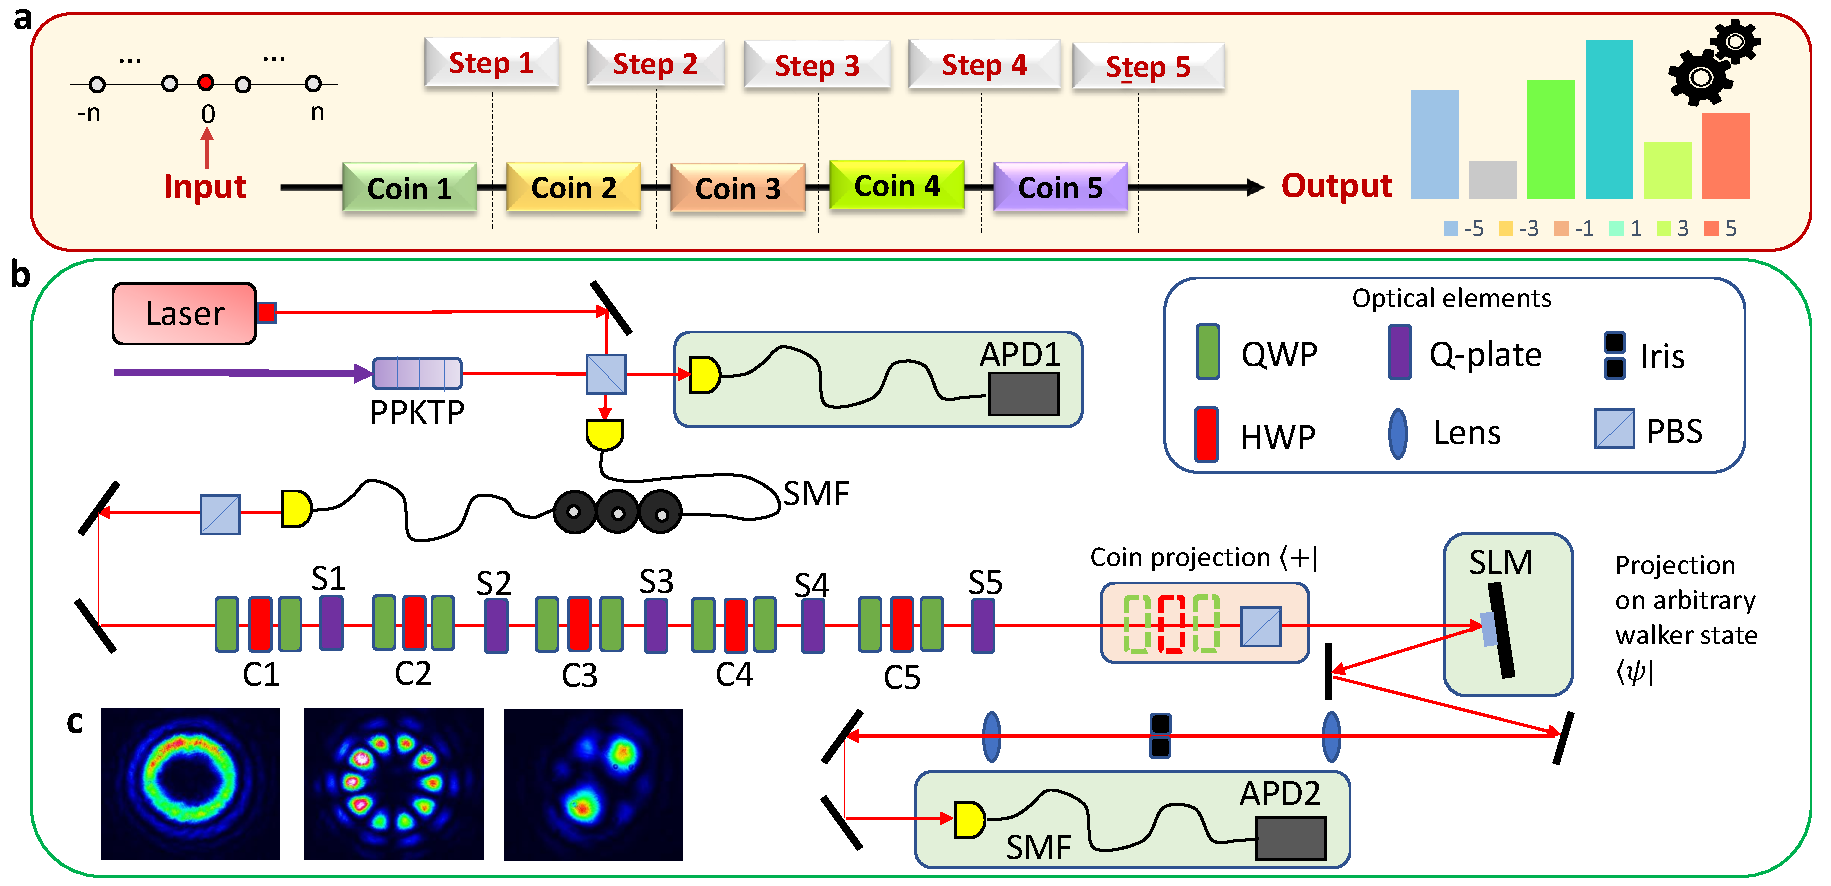
\includegraphics[width=\textwidth]{experimental-QSE-1.pdf}
\caption{
	Setup for the quantum state engineering toolbox.
	\textbf{(a)} Conceptual scheme of the protocol. At each step of \ac{QW} the coin operator is changed to obtain a target state in the output.
	\textbf{(b)} A single-photon source, composed of a \ac{PPKTP} crystal, generates pairs of photons that are coupled in a single-mode fibre (SMF). One photon acts as trigger while the other is prepared in $\ket{\psi_0}=\ket{+}\otimes \ket{0}$ through polarisation controllers and a \ac{PBS}. Five sets of \acp{QWP} and \acp{HWP} \highlight{check acronyms} implement operators $\{ C_i\}_i$ for each step. Five \acp{QP} implement the shift operator of the \ac{QW} $\{S_i\}$.
	The detection stage consists of a \ac{PBS} followed by a \ac{SLM}, a \ac{SMF} and an \ac{APD}, for projection onto $\ket{+} \otimes \ket{\psi}$.
	\textbf{(c)} Pictures of \ac{OAM} modes of the output states after \ac{PBS}, obtained with coherent light. From right: \ac{OAM} eigenstate corresponding to $m=5$; balanced superposition of $m=\pm 5$; balanced superposition of all \ac{OAM} components covered by 5-step \ac{QW} $m=\{\pm 5, \pm 3, \pm 1\}$.
}
\label{fig:expQWs:schematics}
\end{figure}


\tmpHeading{How are QW operations implemented physically?}
Single-photon states are generated via a type-II, collinear \ac{SPDC} source (see~\cref{fig:expQWs:schematics}).
The photons emitted by the source are separated with a \acf{PBS} and coupled to two \acfp{SMF}. One photon acts as the trigger signal, while the other one undergoes the \ac{QW} evolution. After the propagation in the \ac{SMF} and the first \ac{PBS}, the state of the photons is $\ket{\psi_0}_{wc}=\ket{0}_w \otimes \ket{+}_c$ where $\ket{+}_c=(\ket{{\uparrow}}_c+\ket{{\downarrow}}_c)/\sqrt2$. After $n$ steps, the protocol involves a projection of the coin state onto $|+\rangle_c$, experimentally implemented by a final \ac{PBS}.
To reconstruct the generated \ac{OAM} states, the light is coupled into a \ac{SMF} after passing through a \ac{SLM}.
This allows to measure arbitrary \ac{OAM} states with high accuracy~\cite{bolduc2013exact,dambrosio2013test}.
The state fidelity between generated and target states is estimated by projecting the \ac{OAM} state onto a basis containing the target state (see~\cref{fig:expQWs:schematics}).



\tmpHeading{Other possible QSE schemes}
Among other possible architectures for quantum state engineering are intrinsically-stable bulk interferometric schemes~\cite{broome2010discrete,kitagawa2012observation,vitelli2013joining}.
In this approach, the coin is implemented in the polarisation degree of freedom,
while the shift operator is performed by introducing a spatial displacement of the optical mode conditionally to the polarisation state of the photon.
Other approaches include integrated linear interferometers~\cite{sansoni2012twoparticle, crespi2013anderson, harris2015bosonic, pitsios2016photonic}, and fiber-loops architectures~\cite{schreiber2010photons, schreiber2012a, boutari2016large}. As mentioned, besides purely optical settings, one could envisage to adapt the present protocol to other physical systems that can host quantum walks \cite{manouchehri2014physical}, such as trapped atoms \cite{karski2009quantum} and ions \cite{schmitz2009quantum, zhringer2010realization} as well as cold atoms in lattices \cite{weitenberg2011singlespin, fukuhara2013microscopic, preiss2015strongly}.

\tmpHeading{Advantages of using OAM}
The encoding of quantum dynamics in the angular momentum degree of freedom has several advantages, including the possibility to generate and manipulate quantum states in high dimensions~\cite{fickler2012quantum,dambrosio2013photonic}. In the context of quantum walks, encoding of coin and position in the \ac{SAM} and \ac{OAM}, respectively, has the crucial property to avoid the requirement of an interferometric scheme. This guarantees an intrinsic phase stability, since all the evolution is inside the same light beam. Furthermore, the approach employed in this platform leads to a linear scaling in the number of optical elements with respect to the number of steps, and thus to the Hilbert space dimension~\cite{cardano2015quantum}.

\tmpHeading{Scaling of the platform}
Experimental limitations in the maximum achievable number of steps are due to the generation process of \ac{OAM} eigenstates by the \acp{QP}. To prevent coupling between the radial and azimuthal parts of the beam during the propagation in free space, all of the evolution has to happen in the near-field regime~\cite{karimi2009light,cardano2015quantum}. This means that the distance $\ell$ between consecutive \acp{QP} has to such that $\xi\equiv \ell/z_R \ll 1 $, where $z_R$ is the Rayleigh range.
In our setup, the employed beam waist $w_0$  ensures a $z_R> \SI{30}{\meter}$ at wavelength $\lambda=\SI{808}{nm}$. Two adjacent \acp{QP} are separated by a distance $\ell \sim \SI{15}{cm}$ (such distance is needed to insert, between the \acp{QP}, the waveplates implementing the coin), such that the condition on $\xi$ is satisfied.  Furthermore, in this regime the Gouy phase can be neglected allowing a good control of the coherence between different \ac{OAM} components, and, consequently, on the output states. However, in the perspective of higher number of steps, the requirement to have a $z_R$ large at least as the total length $L$ of the platform also implies a large beam waist, thus limiting the maximum amount of steps that can be implemented. An alternative strategy could be to use a loop scheme, where consecutive steps are performed by multiple passes through the same \ac{QP} and waveplates~\cite{goyal2013implementing}. In this alternative setup, a suitable $4f$ lens system is necessary to image the output of the q-plate at the input of the next step, being such approach equivalent to work in the near-field regime.  
In this combined \ac{OAM}-loop scheme, experimental challenges arise at the measurement stage, that in spin-\ac{OAM} setup involves a \ac{SLM}. When integrating such encoding in a loop-architecture, issues may arise due to their slow response time.

\begin{figure}[tb]
\centering
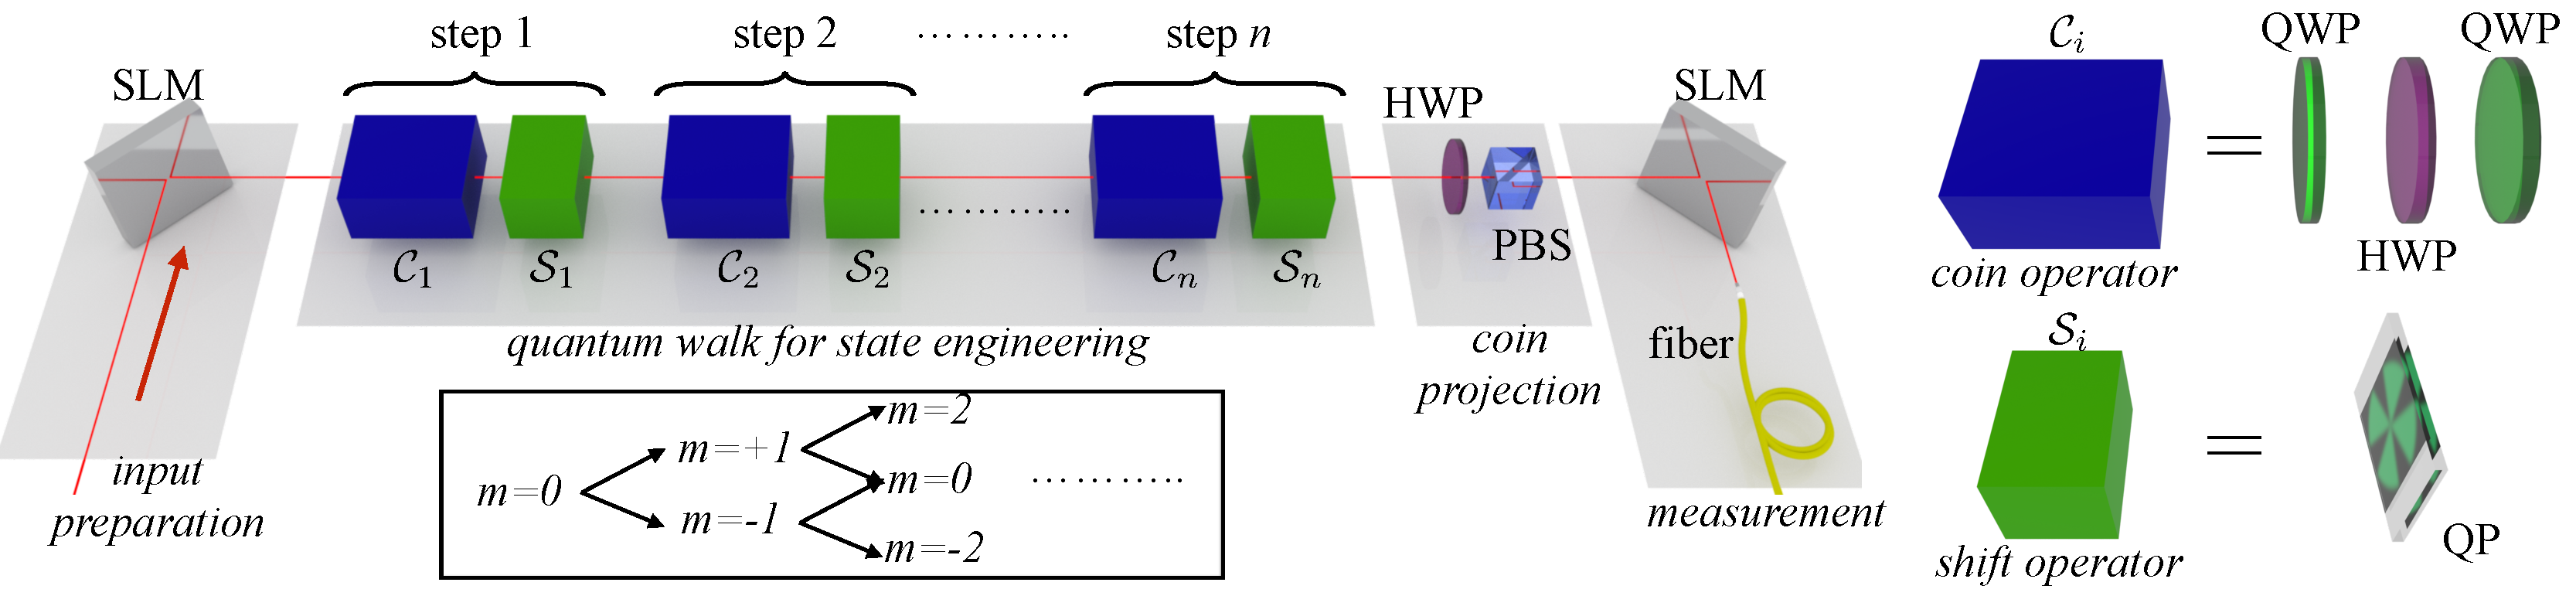
\includegraphics[width=0.99\textwidth]{experimental_apparatus_scheme.pdf}
\caption{\highlight{to fix and reference}
    Scheme for the proposed implementation of the quantum walk state engineering protocol using Orbital Angular Momentum (\ac{OAM}) and Spin Angular Momentum of a photon.
    The input state is prepared in a superposition of $n$ modes with a Spatial Light Modulator (SLM).
    At each step, the coin operation is then realised in polarisation with a sequence of a Quarter Wave Plate (QWP), a Half Wave Plate (HWP) and a second QWP, arranged to implement an arbitrary transformation.
    The shift operation in \ac{OAM} space is implemented with a q-plate (QP), which shifts the \ac{OAM} of $\pm 2q$ conditionally to the polarisation state of the photon.
    For $q=1/2$, the shift is equal to $\pm 1$, with the corresponding evolution is  schematically shown in the lower box.
    Finally, the coin is projected in the $\vert + \rangle$ state by means of a HWP and a polarising beam splitter (PBS).
    A second SLM followed by a single-mode fiber performs the measurement of the output state.
}
\label{fig:QWs:proposal_exp}
\end{figure}


\section{Engineering arbitrary qudits}
\label{sec:expQWs:arbitrary_qudits}

\tmpHeading{Types of generated states}
To demonstrate the flexibility of the protocol, we showcase the generation of a variety of states, including: cat-like states (see~\cref{subsec:expQWs:catstates}), \acp{SCS} (see~\cref{subsec:expQWs:SCSs}), completely balanced states, Fourier basis states, and randomly sampled states.
% from balanced to completely randomly states.
% Balanced states are challenging as one needs to ensure equal population of all their components, a condition that is very prone to experimental imperfections.
% Assessing the quality of generation of such states provides a significant benchmark to the effectiveness of the procedure.

We also engineer the components of the Fourier basis associated to the Hilbert space of the walker. This choice is motivated by the importance of the quantum Fourier transform in quantum algorithms \cite{nielsen2002quantum}, as well as its role in identifying mutually unbiased bases for quantum cryptography and communication in high-dimensions~\cite{durt2010mutually,bandyopadhyay2002new,brierley2009constructing,dambrosio2013test}.

\tmpHeading{Results}
Final measurements concern the generation of randomly-chosen qudits. We have engineered up to $5$ states with real-valued amplitudes and 5 with complex-valued ones, where the state components are sampled from a uniform distribution (cf. Ref.~\cite{SI}).
In~\cref{fig:VVBs:figSpin}\textbf{f}, we report the fidelities for all the experimentally engineered states.
% , including the Fourier basis \highlight{???} and the randomly sampled qudits,
The red area shows the average fidelity and its uncertainty ($\mathcal{F}{=}0.954 \pm 0.001$)~\cite{SI}. Such test provides further evidence of the effectiveness of our engineering strategy.

\begin{figure}[tb]
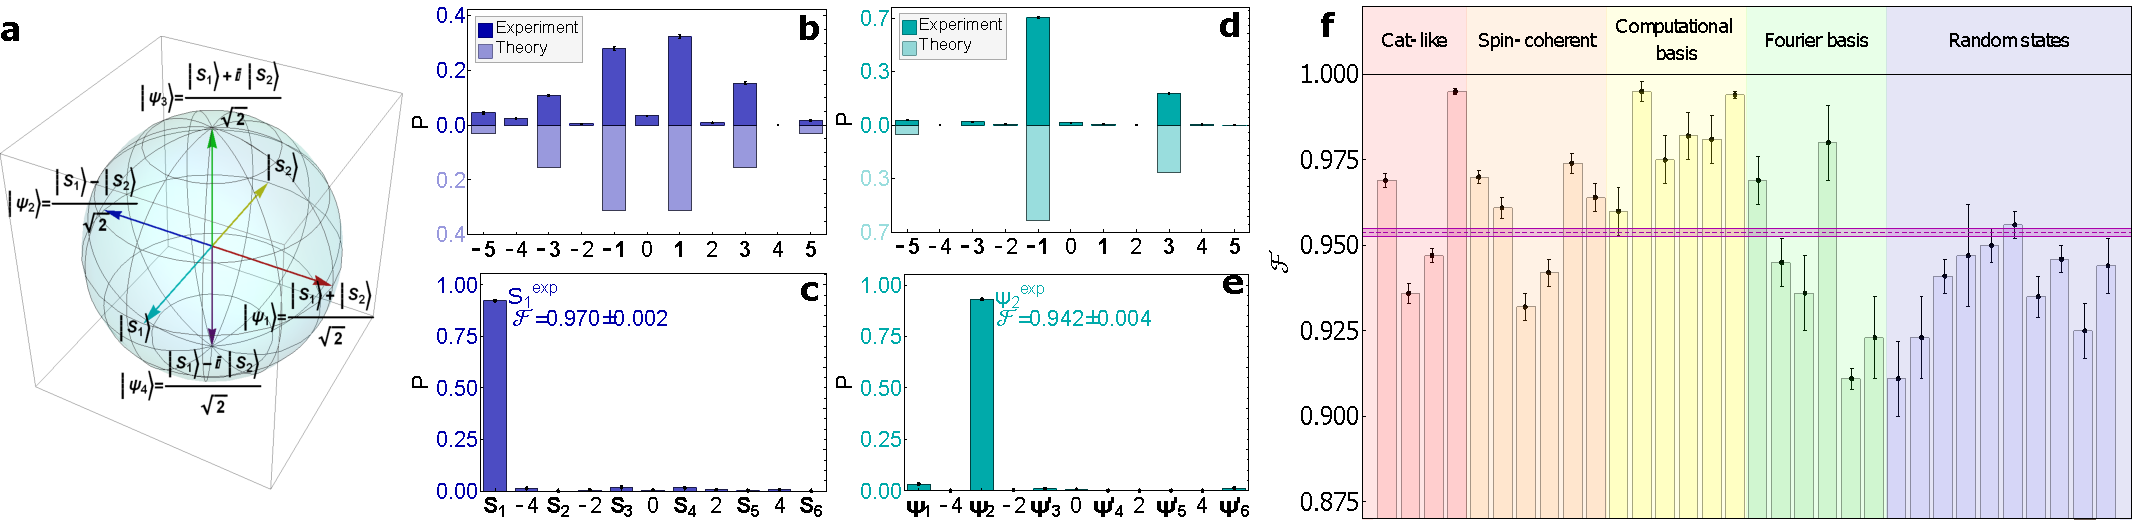
\includegraphics[width=\textwidth]{experimental-QSE-3.pdf}
\caption{
	Experimental results for the engineering of \acp{SCS} and their coherent superposition:
	\textbf{(a)} Bloch-sphere representation for the mutually orthogonal \acp{SCS} $\ket{S_1}$ and $\ket{S_2}$.
	\textbf{(b)} Probability distributions associated to the projection of $\ket{S_1}$ onto the computational basis. As previously explained, we also consider the contribution of even \ac{OAM} components.
	\textbf{(c)} Probability distribution corresponding to the basis that contains the target state itself $\ket{S_1}$, generated with the fidelity reported in the panel. Such orthonormal basis, $\{S_i\}_i$ with $i=1 ...6$, contains eigenstates of $\hat{S}_x$ for a particle with spin $s=5/2$ that are in turn all spin-coherent states.
	\textbf{(d)} Experimental probability distribution on computational basis for $\ket{\psi_2}=\frac{1}{\sqrt{2}}\left(\ket{S_1}- \ket{S_2} \right)$. Only components $\{-5, -1, 3\}$, corresponding to logical states $\{1,3,5\}$, have non-zero probabilities.
	\textbf{(e)} Quantum state fidelity evaluated measuring state $\ket{\psi_2}$ on the orthonormal basis that contains state $\ket{\psi_1}$, as described in the main text. 
	\textbf{(f)} Summary of quantum state fidelities for the $32$ states generated in the experiment. The average fidelity, $\bar{\calF}=0.954\pm 0.001$, is reported by the magenta area.
}
\label{fig:VVBs:figSpin}
\end{figure}

\subsection{Cat-like states}
\label{subsec:expQWs:catstates}

\tmpHeading{What do we mean by ``cat-like states''}
\emph{Cat-like states} are coherent superpositions of two extremal sites of the walker, that is, states of the form $\alpha\ket{5}+\beta\ket{-5}$. The isomorphism of the \ac{OAM} with an angular momentum of quantum number $n/2$ allows to put in correspondence the position states $\ket{\pm 5}$ of the walker with angular momentum states with minimum and maximum projections onto the quantisation axis $\ket{\pm 5/2}$ (for simplicity of notation, we will use position states only). Such isomorphism makes a coherent superposition state such as $(\ket{5}+e^{i\varphi}\ket{-5})/\sqrt{2}$ (with $\varphi$ a suitable phase) into a faithful angular momentum Schrödinger cat state~\cite{militello2006distilling}, thus benchmarking the performance of our experiment with a relevant class of states~\cite{chandrashekar2008optimizing,zhang2016creating,majury2016robust} used in quantum sensing~\cite{fickler2012quantum,dambrosio2013photonic}.

\tmpHeading{Experimental results}
In~\cref{fig:expQWs:results} we report the experimental results for the generation of four cat-like states., which are conveniently pictured as states pointing towards the poles of a Bloch-like ball \highlight{(???)}. Quantum coherence between the components of such states has been tested by changing their relative phase. The values of the state fidelity between experimentally synthesised states and their respective target ones are reported in~\cref{fig:expQWs:results}. Hereafter we compute fidelities by projecting the state on the orthonormal basis which includes the target qudit in the 6-dimensional subspace associated to our 5-step \ac{QW}, generated by \ac{OAM} eigenstates $\{|m\rangle_w\}$ ($m=\pm 5, \pm 3, \pm 1$).

\begin{figure}[tb]
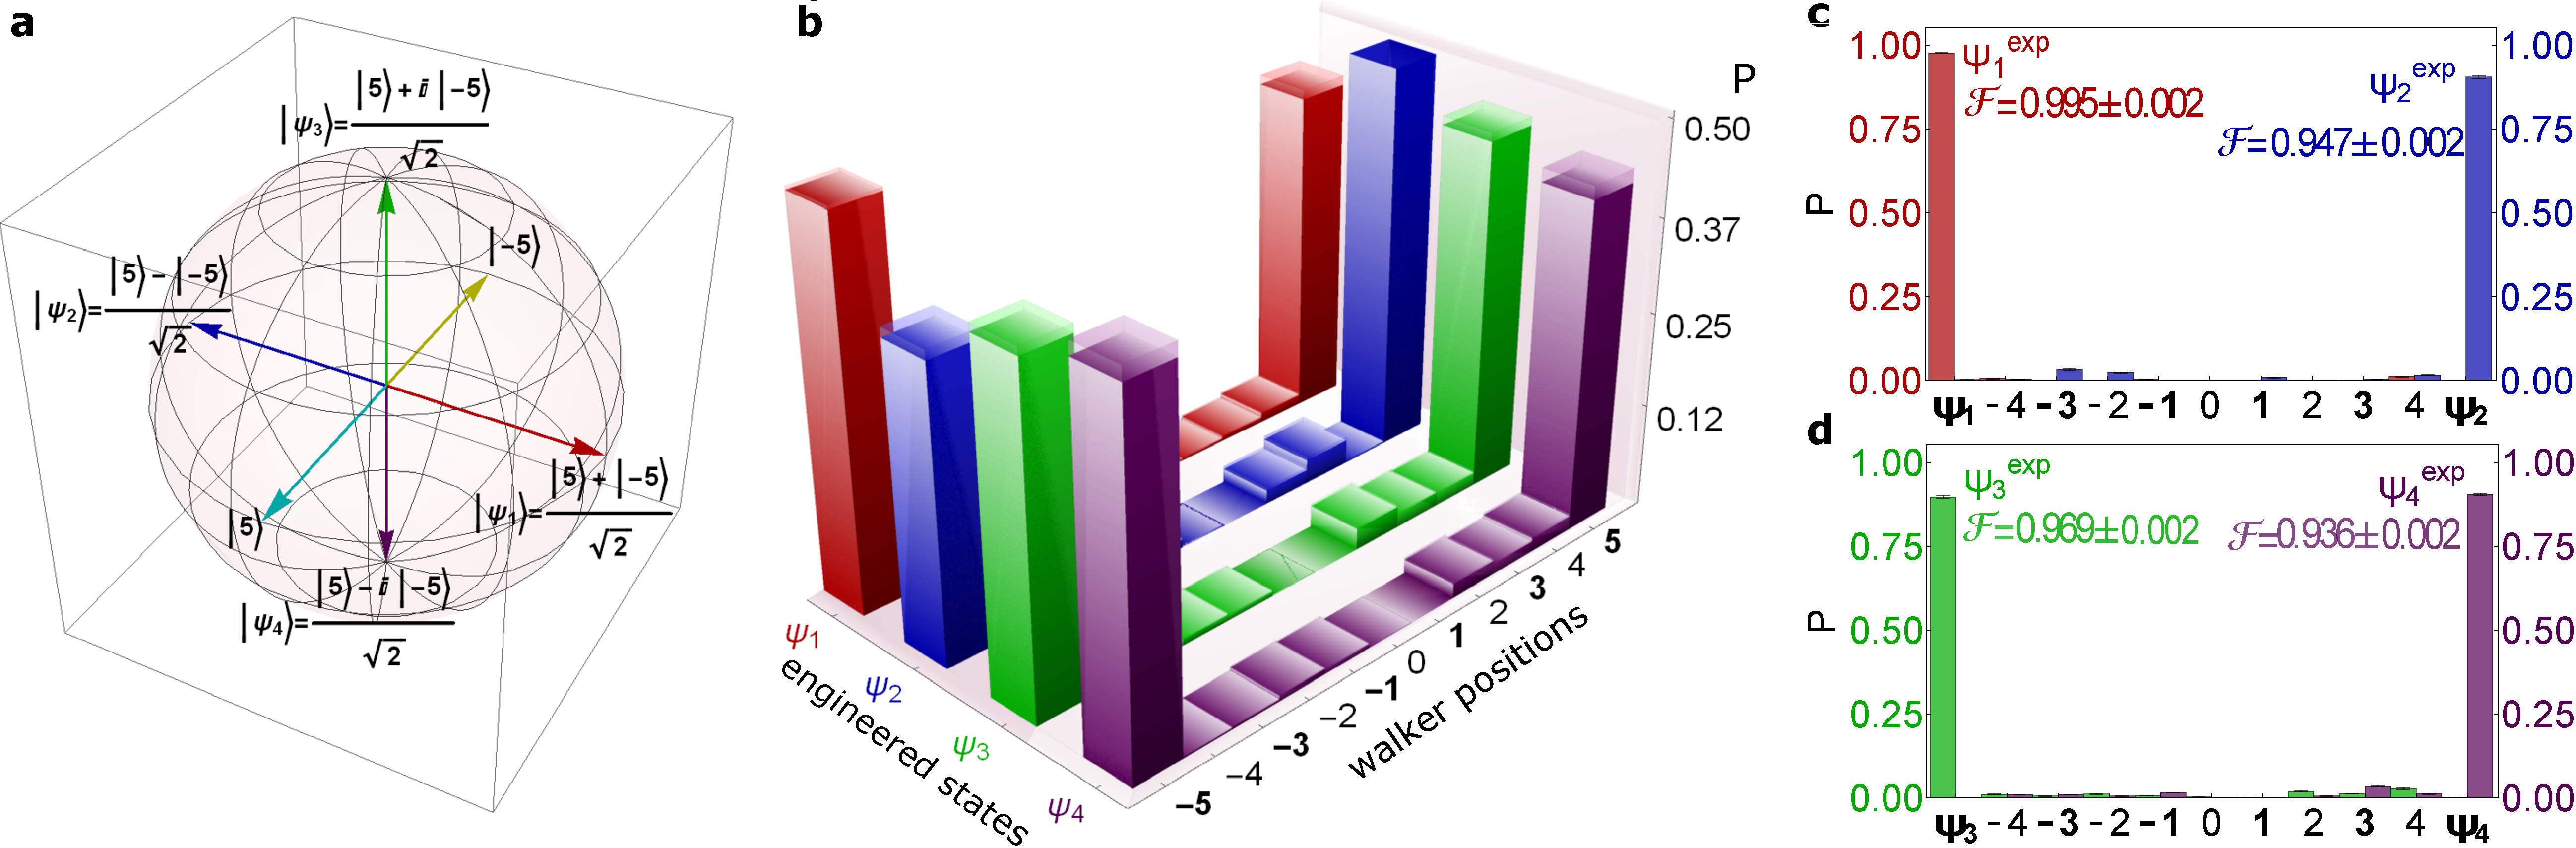
\includegraphics[width=\textwidth]{experimental-QSE-2.pdf}
\caption{
	Experimental results for the engineering of angular momentum cat states.
	\textbf{(a)} Representation on a Bloch-like ball of the four target states corresponding to the superposition of $\ket{\pm 5}$, which correspond corresponding to \ac{OAM} states with maximum and minimum projection of the angular momentum along the quantisation axis.
	\textbf{(b)} Population of the \ac{OAM} components after 5-step {QW} for the states $\ket{\psi_i}~(i=1,2,3,4)$ in panel {\bf a}. Odd-$m$ position states (bold numbers on $x$-axis) should be the only ones involved in the state engineering. However, we report also the populations of even-$m$ position states (light-black numbers on $x$-axis) to illustrate possible imperfections at generation and detection stages. The error bars associated with experimental populations are shown by the transparent areas on top of each histogram.
	\textbf{(c)-(d)} Distributions of probabilities $P_i=\langle B^{(j)}_i\vert\rho_\text{exp}\vert B^{(j)}_i\rangle~(j=1,2)$ that the experimental walker state $\rho_\text{exp}$ is found to be one of the elements of the bases $B^{(j)}=\{\ket{\psi_p},\ket{\psi_{p+1}},\ket{\pm4},\ket{\pm3},\ket{\pm2},\ket{\pm1},\ket{0}\}$ with $p=1$ for $j=1$ and $p=3$ for $j=2$. All the error bars are due to Poissonian uncertainties, propagated through Monte Carlo methods. The state fidelities ${\cal F}$ are calculated as described in the main text.
}
\label{fig:expQWs:results}
\end{figure}

\subsection{Spin-coherent states}
\label{subsec:expQWs:SCSs}

A second class of states considered are \acp{SCS}~\cite{agarwal1997atomic}.


\tmpHeading{What are SCSs?}
\acfp{SCS} are the counterparts of coherent states of the harmonic oscillator for a particle with spin $s$~\cite{radcliffe1971some,arecchi1972atomic,agarwal1997atomic,markham2003classicality}. They are eigenstates -- with eigenvalue $s$ -- of the component of the total spin-momentum operator $S_{\theta,\phi}$ along the direction identified by the spherical angles $(\theta, \phi)$~\cite{arecchi1972atomic,agarwal1997atomic,ulyanov1999spin,lee2015visualizing}.
A decomposition of such states over the $\{\ket{m}\}$ basis of the projected spin along the $z$-direction, $S_z$, reads
\begin{equation}
\begin{aligned}
	\ket{s,\theta,\phi} &=
		\sum_{m=-s}^{s}
		\sqrt{\frac{(2s)!}{(s+m)!(s-m)!}} e^{-i\phi m} C_\theta^{s+m} S_\theta^{s-m}\ket{m},
\end{aligned}
\label{spin_coherent1}
\end{equation}
with $C_\theta\equiv\sqrt{1-S^2_\theta}=\cos(\theta/2)$. \acp{SCS} have numerous applications in condensed matter physics, in particular for quasi-exactly solvable models, for the Wigner-Kirkwood expansion and in quantum correction to energy quantisation rules~\cite{ulyanov1999spin}. At a more foundational level, they can be used to generate Schrödinger cat states~~\cite{agarwal1997atomic}. 

\tmpHeading{Some background math}

Although \acp{SCS} are in general not orthogonal, they form a convenient basis. Moreover, as two \acp{SCS} pointing in opposite azimuthal directions are orthogonal for $\theta\sim\pi/2$, by restricting the attention to $\{\ket{s,\pi/2,\phi},\ket{s,-\pi/2,\phi}\}$ we would be dealing with an orthonormal basis, which we can use to construct the analogous of a Bloch ball for a two-level system (cf.~\cref{fig:VVBs:figSpin}\textbf{a}). We have thus engineered $\ket{S_1}\equiv\ket{5/2,\pi/2,0}$ and $\ket{S_2}\equiv\ket{5/2,-\pi/2,0}$, and considered the experimental synthesis of balanced coherent superpositions of such states.
Furthermore, $S_1$ and $S_2$ are also eigenstates of the $\hat{S}_x$ operator. In~\cref{fig:VVBs:figSpin}\textbf{b-c} the state $S_1$ is projected firstly on the computational basis, the eigenstates of $\hat{S_z}$, and then on the basis $\{S_i\}$, with $i=1...6$, which consists of $\hat{S}_x$ eigenstates. Balanced superpositions of $S_1$ and $S_2$ are akin to the Schrödinger cat states built on coherent states of a harmonic oscillator, as they exhibit signatures of non-classical interference~\cite{agarwal1997atomic,SI}. For instance, only even (odd) components of the logical basis enter the superposition $\ket{S_1}+\ket{S_2}$ ($\ket{S_1}-\ket{S_2}$), a parity rule that is fully analogous to the one characterizing even (odd) bosonic cat states. Thanks to the isomorphism between the spaces of \ac{OAM} and of arbitrary angular momentum equal to $n/2$, we can generate \ac{SCS} mapping the basis $\{ \ket{s_z}\}$ in (\ref{spin_coherent1}) into the basis of the \ac{QW} $\{|m\rangle_w\}$. The results are illustrated in~\cref{fig:VVBs:figSpin}a-e, where we show the high quality of both the generated \acp{SCS}and \ac{SCS}-based cat states. %In particular, in Fig.\ref{spin_coherent1}.d we observe the odd parity that characterizes the superposition with minus sign.
\highlight{(ritornare su questa roba)}

\subsubsection{Cat states based on spin coherent states: phase-space picture}

The decomposition of a \ac{SCS} $\ket{s,\theta,\phi}$ over the basis of eigenstates of angular momentum $\{\ket{m}\}_{m=-s}^s$ reads
\begin{equation}
	\ket{s,\theta,\phi} =
	\sum^s_{m=-s}
		\sqrt{\frac{(2s)!}{(s+m)!(s-m)!}}
		e^{-i\phi m} C^{s+m}_\theta S^{s-m}_\theta \ket{m},
\end{equation}
with $C_\theta\equiv\sqrt{1-S^2_\theta}=\cos(\theta/2)$. We have also introduced the \ac{SCS}-based Schrödinger cat states built as the following superpositions of orthogonal states $\ket{S_1}:=\ket{5/2,\pi/2,0}$ and $\ket{S_2}:=\ket{5/2,-\pi/2,0}$:
\begin{equation}
%\begin{aligned}
\ket{\psi_{1}}=\frac{1}{\sqrt 2}(\ket{S_1}+\ket{S_2}),\qquad\ket{\psi_{2}}=\frac{1}{\sqrt 2}(\ket{S_1}-\ket{S_2}).
%\end{aligned}
\end{equation}
In this Section, we aim at providing a brief analysis of the features of such states, which are best analyzed in a suitably defined phase space~\cite{agarwal1997atomic}. In particular, we shall be considering the analogous of the Husimi $Q$ function~\cite{walls2007quantum} defined as
\begin{equation}
\label{deco}
Q_j(\alpha,\beta)=\vert\langle{5/2,\alpha,\beta}\vert\psi_j\rangle\vert^2\qquad(j=1,2)
\end{equation}
in the spherical polar space where the Cartesian coordinates $(x,y,z)$ are mapped into $x\to Q_j(\alpha,\beta)\sin\alpha\cos\beta$, $y\to Q_j(\alpha,\beta)\sin\alpha\sin\beta$ and $z\to Q_j(\alpha,\beta)\cos\alpha$. Despite the simplicity of its definition, $Q_j(\alpha,\beta)$ captures important information about the quantum interference between the orthogonal components of $\ket{\psi_{j}}$, which differentiate such states from the incoherent mixture of \acp{SCS} $(\ket{S_1}\bra{S_1}\pm\ket{S_2}\bra{S_2})/2$. 

The orthogonality of $\ket{S_1}$ and $\ket{S_2}$ allows one to cast $Q_j(\alpha,\beta)$ as 
\begin{equation}
Q_j(\alpha,\beta)=\frac12\left(|q_+(5/2,\alpha,\beta)|^2+|q_-(5/2,\alpha,\beta)|^2+\text{sign}_j2\text{Re}[q_+(5/2,\alpha,\beta)q^*_-(5/2,\alpha,\beta)]\right)
\end{equation}
where $q_\pm(s,\alpha,\beta)=\bra{s,\alpha,\beta}{s,\pm\theta,0}\rangle$ and $\text{sign}_1=-\text{sign}_2=+1$. Such scalar products can be evaluated explicitly for any value of $s$ by using the decomposition in Eq.~\eqref{deco} to get 
\begin{equation}
\begin{aligned}
q_\pm(\alpha,\beta)&=(\pm 1)^s\frac{\Gamma (2 s+1)}{\Gamma (s+1)^2} S^s\left({\alpha }\right) C^s\left(\alpha\right) S^s\left(\theta\right) C^s\left({\theta
   }\right) \left[\, _2F_1\left(1,-s;s+1;\mp e^{-i \beta  } T\left({\alpha}\right) T\left({\theta }\right)\right)\right.\\
  &+\left.{}_2F_1\left(1,-s;s+1;\mp e^{i \beta} T^{-1} \left({\alpha}\right) T^{-1}\left({\theta }\right)\right)-1\right],
  \end{aligned}
\end{equation}
where $T(\alpha)=S(\alpha)/C(\alpha)=\tan(\alpha/2)$, $_2F_1(a,b,c;d)$ is the ordinary Hypergeometric function, and $\Gamma(d)$ is the Gamma function with argument $d$. 
\begin{figure}[!t]
    \centering
    {\bf (a)}\hskip8cm{\bf (b)}\\
    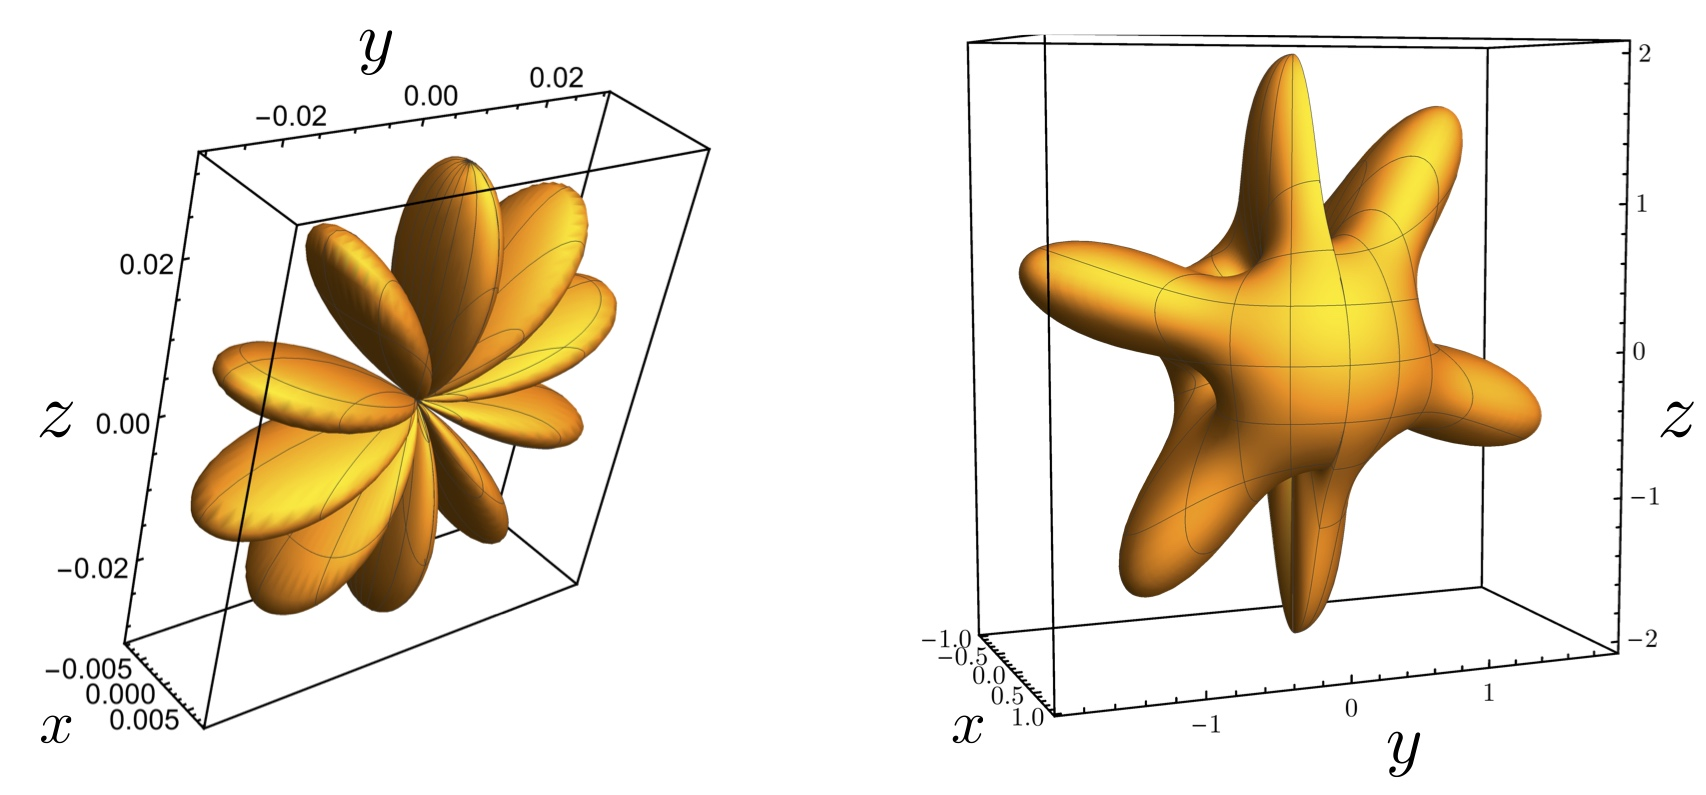
\includegraphics[width=\columnwidth]{experimentalQSE-Insieme.jpg}
    \caption{Spherical polar plot of the interference term $-\text{Re}[q_+(5/2,\alpha,\beta)q^*_-(5/2,\alpha,\beta)]$ in the $Q_2(\alpha,\beta)$ function.}
    \label{insieme}
\end{figure}

Using such expressions, we can compute $Q_j(\alpha,\beta)$ to investigate its features. However, looking at such function directly does not provide sufficient information for the discrimination of an incoherent mixture and a state such as $\ket{\psi-{1,2}}$. On the other hand, we find more informative to consider that $\frac12\left(|q_+(5/2,\alpha,\beta)|^2+|q_-(5/2,\alpha,\beta)|^2\right)$ is precisely the spherical SCS-based $Q$ function for the incoherent state $(\ket{S_1}\bra{S_1}\pm\ket{S_2}\bra{S_2})/2$. Let us call it $Q_{inc}(\alpha,\beta)$, so that 
\begin{equation}
Q_j(\alpha,\beta)=Q_{inc}(\alpha,\beta)+\text{sign}_j\text{Re}[q_+(5/2,\alpha,\beta)q^*_-(5/2,\alpha,\beta)],
\end{equation}
which pinpoints the contribution coming from the fixed-phase relation typical of a coherent superposition. We thus focus on state $\ket{\psi_2}$, which is the one that has been addressed in our experimental endeavors, and look at the term $-\text{Re}[q_+(5/2,\alpha,\beta)q^*_-(5/2,\alpha,\beta)]$, and represent it in the spherical polar plane defined above. Fig.~\ref{insieme} {\bf (a)} shows the results of our calculations. 

Such interference term exhibits 10 equally separated lobes, and is clearly displays both rotation and inversion symmetry. In fact, one can show that, for a generic value of $s$, the interference term in the corresponding $Q$ function exhibits $4s$ equally spaced lobes. It is worth mentioning that in Ref.~\cite{agarwal1997atomic} another figure of merit for the analysis of the effects of the interference term was adopted. More specifically, Ref.~\cite{agarwal1997atomic} studied the form of 
\begin{equation}
\frac{Q_j(\alpha,\beta)}{Q_{inc,j}(\alpha,\beta)}=1+\text{sign}_j\frac{2\text{Re}[q_+(5/2,\alpha,\beta)q^*_-(5/2,\alpha,\beta)]}{Q_{inc,j}(\alpha,\beta)},
\end{equation}
which thus quantifies the effect of quantum coherence as the deviation of $Q_j(\alpha,\beta)$ from $1$, whose representation in the chosen spherical polar space is a sphere of unit radius. When making use of such figure of merit, we find Fig.~\ref{insieme} {\bf (b)}, which shows a lobate behavior significantly different from the (incoherent) spherical trend. 


\subsection{Other engineered states}

In the following table we report the summary of target states engineered during the experiment, with corresponding quantum state fidelities and generation probabilities. The latter are provided by the algorithm developed in Ref.~\cite{innocenti2017quantum}, together with the coin operators needed in the engineering process.
% \add{In  particular  we  observe  that the generation  probability  depends  on  the  target  state.   Concerning balanced states, as the element of Fourier basis, we find the scaling $O(1/2d)$ as reported in \cite{innocenti2017quantum}. The expected theoretical fidelity for all states is 1, independently from the size of the quantum walk.}
The protocol and the experimental platforms are tested firstly with the elements of the computational basis corresponding to the eigenstates of the \ac{OAM}, here denoted as $\{\ket{m} \}=\{\ket{\pm5}, \ket{\pm3},\ket{\pm1} \}$. We then consider superpositions of two computational basis states, and then proceed with more complex states such as spin-coherent states, the elements of the Fourier basis, and lastly random states. The quantum state fidelities are calculated measuring the target state on an orthonormal basis, generated via Gram-Schmidt orthogonalization, which contains the state itself.

Let us clarify the notation used in Table~\ref{table:expQWs:summary}. For the Fourier basis the convention employed is the following: $\ket{\on{QFT}_k}=\frac{1}{\sqrt{6}}\sum_{j=1}^{6}e^{\frac{ i \pi jk }{3}}\ket{j}$, where $\{\ket{j}\}$ stands for the logical basis that in our case corresponds to the \ac{OAM} eigenstates $\{\ket{m} \}$. The notation $\ket{r_k}$ and $\ket{c_k}$ refers to real and complex random states respectively. Amplitudes of real states have been sampled uniformly in the range $\left[0,1\right]$ and then normalized. In the case of complex states we have sampled the real and imaginary part separately in the range $\left[-0.5,0.5\right]$. In Table~\ref{table:expQWs:random_states_amps} we report the resulting amplitudes.

\begin{table}[tbh]
\centering\footnotesize
\begin{tabular}{lcc|lcc}
\toprule
Target State & $Probability$  & $\mathcal{F}_{exp}$  & Target State & $Probability$  & $\mathcal{F}_{exp}$ \\
\midrule
 $\quad\ket{-5}$ & $0.5$  & $0.981 \pm 0.007\quad$ &$\quad\ket{\on{QFT}_1}\qquad $ & $0.14$ & $0.969\pm 0.007$\\
 $\quad\ket{-3}$ & $0.5$ & $0.982 \pm 0.007\quad$ &$\quad\ket{\on{QFT}_2}$ & $0.17$ & $0.923\pm 0.022$ \\
 $\quad\ket{-1}$ & $0.5$ & $0.960 \pm 0.007\quad$ &$\quad\ket{\on{QFT}_3}$ & $0.17$ & $0.911\pm 0.011$\\ 
 $\quad\ket{1}$ & $0.5$ & $0.995 \pm 0.007\quad$ & $\quad\ket{\on{QFT}_4}$&$0.17$ &  $0.980\pm 0.011$ \\
 $\quad\ket{3}$ & $0.5$ & $0.975 \pm 0.007\quad$ & $\quad\ket{\on{QFT}_5 }$& $0.17$& $0.936\pm 0.011$ \\
 $\quad\ket{5}$ & $0.5$ & $0.994 \pm 0.001\quad$ & $\quad\ket{\on{QFT}_6} $& $0.17$ & $0.945\pm 0.007$ \\
 $\quad\frac{1}{\sqrt{2}}\left(\ket{-5}+\ket{5} \right)$ & $0.5$  & $0.995 \pm 0.001\quad$ &$\quad\ket{r_1}$ & 0.22& $0.911\pm0.011$\\
 $\quad\frac{1}{\sqrt{2}}\left(\ket{-5}-\ket{5}\right)$ & $0.5$ & $0.947 \pm 0.002\quad$ &$\quad\ket{r_2}$  & 0.16 & $0.923 \pm 0.012$\\
 $\quad\frac{1}{\sqrt{2}}\left(\ket{-5}+i\ket{5}\right)$ & $0.5$ & $0.969 \pm 0.002\quad$ &$\quad\ket{r_3}$  & 0.17 & $0.941 \pm 0.004$\\ 
  $\quad\frac{1}{\sqrt{2}}\left(\ket{-5}-i\ket{5}\right)$ & $0.5$ & $0.936 \pm 0.003\quad$&$\quad\ket{r_4} $& 0.14 &$0.947 \pm 0.015$  \\
 %$\frac{1}{\sqrt{2}}\left(\ket{-3}+\ket{3}\right)$ & $0.5$ & $0.912 \pm 0.004$ \\
 $\quad\ket{S_1}=\ket{5/2,\pi /2,0}$   & $0.15$ & $0.970 \pm 0.002\quad$ &$\quad\ket{r_5}$ & 0.19 & $0.950\pm0.005$  \\
 $\quad\ket{S_2}=\ket{5/2,-\pi /2,0}$ & $0.15$ & $0.961 \pm 0.003\quad$ &$\quad\ket{c_1}$ &0.16 & $0.956\pm0.004$ \\
 $\quad\frac{1}{\sqrt{2}}\left(\ket{S_1}+\ket{S_2}\right)$ & $0.15$ & $0.932 \pm 0.004\quad$&$\quad\ket{c_2}$ & 0.29 &$0.935 \pm 0.006$  \\
 $\quad\frac{1}{\sqrt{2}}\left(\ket{S_1}-\ket{S_2}\right)$ & $0.15$ & $0.942 \pm 0.004\quad$& $\quad\ket{c_3}$& 0.17 & $0.925\pm 0.008$ \\
$\quad\frac{1}{\sqrt{2}}\left(\ket{S_1}-i\ket{S_2}\right)$ & $0.23$ & $0.974 \pm 0.003\quad$&$\quad\ket{c_4}$ & 0.16 & $0.944\pm0.008$\\
$\quad\frac{1}{\sqrt{2}}\left(\ket{S_1}+i\ket{S_2}\right)$ & $0.23$ & $0.964 \pm 0.004\quad$& $\quad\ket{c_5}$ & 0.28 & $0.946\pm0.004$\\
\bottomrule
\end{tabular}
\caption{%
	Summary of the measured states with relative generation probabilities and experimental quantum state fidelities.
	\highlight{fix horrible formatting}%
}
\label{table:expQWs:summary}
\end{table}

\begin{table}[tbh]
\centering\footnotesize
\begin{tabular}{cc}
\toprule
State & Amplitudes \\
\midrule
$\qquad\ket{r_1}\qquad$& $\left( 0.51, 0.27, 0.13, 0.10, 0.29, 0.75\right)$\\
$\qquad\ket{r_2}\qquad$& $\left( 0.19, 0.40, 0.04, 0.53, 0.37, 0.62\right)$\\
$\qquad\ket{r_3}\qquad$&$\left( 0.50, 0.74, 0.40, 0.16, 0.10, 0.006\right)$ \\
$\qquad\ket{r_4}\qquad$& $\left( 0.50, 0.47, 0.55, 0.31, 0.36, 0.04\right)$ \\
$\qquad\ket{r_5}\qquad$& $\left( 0.24, 0.12, 0.72, 0.16, 0.54, 0.30\right)$ \\
$\qquad\ket{c_1}\qquad$& $\left( 0.04+0.35i, 0.34+0.41i, 0.10+0.42i, 0.18-0.26i, 0.11-0.11i, -0.47+0.22i\right)$  \\
$\qquad\ket{c_2}\qquad$& $\left( 0.19-0.33i, -0.43+0.30i, -0.18-0.02i, -0.37+0.42i, -0.12-0.10i, 0.23+0.38i\right)$\\
$\qquad\ket{c_3}\qquad$& $\left( -0.19-0.30i, -0.02+0.39i, 0.30-0.15i, 0.25-0.22i, -0.13+0.42i, 0.24+0.48i\right)$\\
$\qquad\ket{c_4}\qquad$& $\left( 0.06+0.07i, 0.30-0.37i, -0.23+0.08i, 0.11-0.13i, -0.22+0.57i, 0.07-0.54i\right)$\\
$\qquad\ket{c_5}\qquad$& $\left( 0.07+0.14i, 0.48-0.34i, -0.41-0.18i, -0.41-0.09i, -0.10+0.32i, 0.32+0.18i\right)$\\
\bottomrule
\end{tabular}
\caption{Amplitudes of random states.}
\label{table:expQWs:random_states_amps}
\end{table}


\section{Behaviour of projection probabilities}
\label{sec:expQWs:projection_probs}

\tmpHeading{In this section...}
In this section we provide a qualitative discussion about the relationship between projection probabilities and the quantum walk steps~\cite{innocenti2017quantum}.

\tmpHeading{The same target can correspond to multiple projection probabilities}
Note that, as was already discussed in~\cref{sec:QWs:focusing_walker_states}, there can be multiple \ac{QW} dynamics that, after suitable projection of the coin, produce a given target state.
These different solutions will, in general, correspond to different projection probabilities.
However, for more than five steps, a general method to compute the full set of solutions is not known, and solutions have to be found via a numerical optimisation~\cite{innocenti2017quantum}.
This method, while computationally more efficient, only produces one of the possible solutions, and thus not necessarily the solution corresponding to the optimal projection probability.
Nonetheless, we find that the projections probabilities obtained by running such numerical optimisation remain $\ge 15\%$ for up to $20$ steps of our protocol. 

\tmpHeading{Estimate the scaling of projection probabilities}
In~\cref{fig:expQWs:avgProbabilitiesVsStepNumber} we give the \textit{average} projection probability as a function of the number of steps. These probabilities are calculated by averaging the projection probabilities obtained by running the optimisation algorithm over uniformly sampled random states, for various numbers of steps. We find the average projection probability to decrease roughly linearly with the number of steps. If we assume this linear decrease to also hold for larger numbers of steps, the average projection probability would be dropping to $\sim 0.1$ at around $25$ steps, that is, for target qudit states of dimension $26$.
It is, however, important to note that this data grossly underestimates the real average probabilities. Indeed, as already mentioned, the optimisation method used here only finds one among many solutions for a given target, and thus generally not the optimal one. Moreover, increasing the step number also increases the number of paths with which a state can be generated, which means that, with this method, we can expect the underestimation to be even more significant for larger step numbers.
Further evidence suggesting that this method underestimates the real average probabilities is obtained by computing the full set of solutions and taking the optimal one, which can be done for up to five steps. Indeed, as shown in~\cref{sec:QWs:numerical_fid_max}, with this method we find the real optimal average probabilities for three, four, and five steps to be consistently $\sim 0.33$, with no detectable decreasing behaviour.

\begin{figure}[tb]
    \centering
    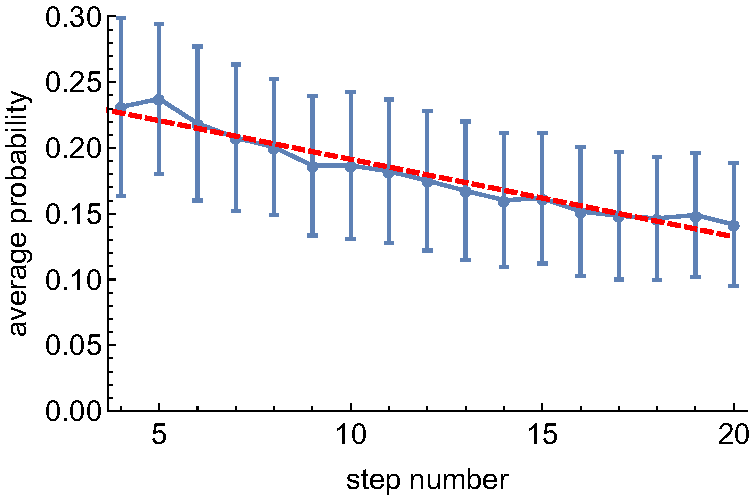
\includegraphics[width=0.8\linewidth]{experimentalQSE-averagesAndVariances_rerundata_manysteps.pdf}
    \caption{
    	Average projection probability obtained for randomly sampled target states with different numbers of steps. Each point corresponds to an average over a sample of $2000$ uniformly sampled random target states of the given dimension. For each target, an optimisation algorithm is used to find a solution producing it, as discussed in~\cref{sec:QWs:numerical_fid_max}. The error bars represent the standard deviation associated with each point. The red dashed line is a linear fit. It should be noted that, as discussed in~\cref{sec:QWs:numerical_fid_max}, this data provides only a lower bound to the real average probabilities.%
    }
    \label{fig:expQWs:avgProbabilitiesVsStepNumber}
\end{figure}


\section{Conclusions}
\label{sec:expQWs:conclusions}

We provided an experimental demonstration of the \ac{QW}-based state engineering scheme described in~\cref{chapter:quantum_walks}, using a photonics apparatus with \ac{OAM} and polarisation as the degrees of freedom of the \ac{QW}.
More specifically, we implemented a five-step \ac{QW}, with full control on the preparation, choice of coin operations, and detection stages. To showcase the effectiveness of the protocol, we demonstrated the synthesis of a number of classes of states.
Our results reinforce the idea that numerical optimization complementing a complex \ac{QW} dynamics is effective for high-dimensional state engineering.
% A natural generalisation of this novel paradigm could be the engineering in the multipartite scenario, exploiting quantum correlations between multiple walkers. Regarding the research of the coin, further improvements of our approach can be envisaged by identifying appropriate routines to optimize the state engineering process in the presence of actual experimental imperfections.
% To this end, machine learning algorithms can be a promising add-on to our numerical optimization approach to adapt the coin operators to a given experimental implementation.
